\documentclass[10pt,conference]{IEEEtran}
\IEEEoverridecommandlockouts

\usepackage{cite}
\usepackage{amsmath,amssymb,amsfonts,amsthm}
\usepackage{algorithm}
\usepackage{algpseudocode}
\usepackage{graphicx}
\usepackage{textcomp}
\usepackage{booktabs}
\usepackage{array}
\usepackage{multirow}
\usepackage{url}
\usepackage{xcolor}
\usepackage{tikz}
\usepackage{pgfplots}
\pgfplotsset{compat=1.18}
\usetikzlibrary{shapes.geometric, arrows.meta, positioning, calc, patterns, fit, backgrounds}

\definecolor{googleblue}{RGB}{26, 115, 232}
\definecolor{googlered}{RGB}{217, 48, 37}
\definecolor{googleyellow}{RGB}{249, 171, 0}
\definecolor{googlegreen}{RGB}{30, 142, 62}
\definecolor{bordergray}{RGB}{189, 193, 198}
\definecolor{codebg}{RGB}{248, 249, 250}

\newtheorem{theorem}{Theorem}
\newtheorem{lemma}{Lemma}
\newtheorem{proposition}{Proposition}
\newtheorem{corollary}{Corollary}
\newtheorem{definition}{Definition}
\newtheorem{remark}{Remark}

\begin{document}

\title{Agent-Synapse: Attention-Guided Speculative Tool Prefetching and Microsecond SRAM KV-Cache Checkpointing Across Heterogeneous AI Accelerators}

\author{\IEEEauthorblockN{Aniket Agrawal}
\IEEEauthorblockA{\textit{Google Cloud AI} \\
Google \\
Bangalore, India \\
aniketagrawal@google.com}
}

\maketitle

\begin{abstract}
Autonomous foundation model agents deployed on modern AI accelerators---such as Google Cloud TPU v6e (Trillium) and NVIDIA Blackwell B200---solve complex enterprise workflows by interleaving autoregressive token generation with external Model Context Protocol (FastMCP) tool invocations across distributed graph databases (Cloud Spanner Graph ISO GQL), analytical warehouses (BigQuery SQL), and vector retrieval engines (Vertex AI Search). Under the prevailing serial reasoning-acting paradigm, the accelerator and the network interface card (NIC) execute in strictly mutually exclusive phases: the serving engine waits passively until the autoregressive decoder emits the entire structured tool-call JSON block and the terminal \texttt{</tool\_call>} end-of-sequence (EOS) token before dispatching the outbound RPC over the wire. Consequently, the physical NIC remains idle throughout token decoding, and the multi-terabyte-per-second accelerator HBM/SRAM pipeline subsequently stalls for $200\text{ ms}$--$850\text{ ms}$ awaiting network I/O completion. Yet naive speculative execution of external tools introduces two severe hazards: (i) premature dispatch of non-idempotent state mutations (\texttt{WRITE}/\texttt{DELETE}) corrupts external systems of record when early predictions diverge, and (ii) conventional HBM Key-Value (KV) cache eviction and re-prefill upon a speculative mismatch incurs $15\text{ ms}$--$45\text{ ms}$ of redundant attention compute.

We present \textbf{Agent-Synapse}, a three-stage hardware-software co-designed runtime that overlaps intra-turn autoregressive token decoding with speculative FastMCP network I/O while guaranteeing observational non-interference and microsecond rollback. First, Stage~1 (\emph{Early-Layer Attention Entropy and Logit-Lens Tool Predictor}) monitors intermediate transformer cross-attention heads across Layers $8$--$16$ and projects hidden states through the unembedding matrix to predict idempotent tool identifiers and canonical argument bindings $150\text{ ms}$--$400\text{ ms}$ ($15$--$35$ decode steps) prior to \texttt{</tool\_call>} EOS emission, gated by a finite-sample split-conformal confidence threshold $\tau_{\textnormal{conf}} = 0.82$. Second, Stage~2 (\emph{Speculative FastMCP Wire Pipeline}) dispatches idempotent read and snapshot-sandboxed requests asynchronously over the physical NIC with deterministic wire headers (\texttt{X-Agent-Speculative-Prefetch: True} and \texttt{X-Synapse-Checkpoint-Hash}) while unconditionally blocking non-idempotent \texttt{WRITE}/\texttt{DELETE} mutations. Third, Stage~3 (\emph{Zero-Penalty SRAM KV-Cache Micro-Checkpointing and Canonical AST Equivalence Splicer}) pins a $16$-token-aligned Copy-on-Write (CoW) KV-cache page table descriptor in on-chip SRAM (TPU v6e VMEM/CMEM or NVIDIA B200 Tensor Memory). Upon \texttt{</tool\_call>} EOS emission, Stage~3 evaluates canonical Abstract Syntax Tree (AST) equivalence between the predicted and emitted calls: on an AST match ($89.4\%$ hit rate), it splices the prefetched payload directly into the KV-cache with $0\text{ ms}$ residual network wait whenever lead time exceeds I/O latency; on a mismatch ($10.6\%$), it rolls back the CoW SRAM page-table pointer in $< 12\,\mu\text{s}$ ($p_{50} = 4.2\,\mu\text{s}, p_{99} = 9.8\,\mu\text{s}$) with zero external side effects. Across $N = 1{,}000$ multi-step enterprise agent traces, Agent-Synapse reduces end-to-end tool-calling $p_{99}$ tail latency by $61.8\%$ ($842.0\text{ ms} \to 321.6\text{ ms}$) and $p_{50}$ median latency by $54.3\%$ ($412.0\text{ ms} \to 188.3\text{ ms}$) with $0.00\%$ ($0/250$) unauthorized mutating dispatches.
\end{abstract}

\begin{IEEEkeywords}
Speculative Tool Prefetching, Model Context Protocol (FastMCP), Logit Lens, Split-Conformal Prediction, Copy-on-Write SRAM KV-Cache Checkpointing, Cloud TPU v6e, NVIDIA B200, Observational Non-Interference
\end{IEEEkeywords}

\section{Introduction}
\label{sec:intro}

The transition of Large Language Models (LLMs) from passive conversational interfaces to autonomous, tool-augmented enterprise agents has fundamentally altered the systems bottleneck of production AI infrastructure~\cite{yao2023react, schick2023toolformer, qin2024toolllm, patil2024gorilla, gemini2025report}. In enterprise cloud deployments---spanning financial crime graph investigation on Google Cloud Spanner Graph~\cite{corbett2012spanner, iso2024gql}, petabyte-scale analytical warehouse aggregation on BigQuery Dremel~\cite{melnik2010dremel}, grounded regulatory retrieval on Vertex AI Search, and transactional ERP orchestration via the Model Context Protocol (MCP)~\cite{anthropic2024mcp, wang2025mcpbench, lumer2025scalemcp, gan2025ragmcp}---a single user request routinely triggers $3$ to $12$ sequential tool-calling turns. While hardware accelerator architects have achieved extraordinary gains in raw matrix-multiply throughput and High-Bandwidth Memory (HBM) bandwidth on sixth-generation Google Cloud TPU v6e (Trillium)~\cite{jouppi2023tpuv4} and NVIDIA Blackwell B200 GPUs~\cite{hennessy2019new}, end-to-end agentic wall-clock latency remains dominated by a structural serialization bottleneck at the boundary between neural token decoding and external network I/O.

\subsection{The Serial Decode-to-I/O Stall in Agentic Serving}
Under the standard autoregressive tool-calling lifecycle implemented by contemporary agent frameworks (e.g., ReAct~\cite{yao2023react}, ToolLLM~\cite{qin2024toolllm}, vLLM~\cite{kwon2023efficient}, SGLang~\cite{zheng2024sglang}, and FastMCP~\cite{anthropic2024mcp}), each tool invocation turn executes as a strictly sequential two-phase barrier:
\begin{enumerate}
    \item \textbf{Phase 1 (Autoregressive Syntax Emission):} To invoke a tool $w \in \mathcal{W}$ with structured JSON arguments $\mathbf{a}$, the foundation model must autoregressively decode $K_{\text{call}} \in [25, 60]$ tokens representing the syntactic wrapper (\texttt{<tool\_call>\{"name": "spanner\_graph\_query\_gql", "arguments": \{"graph\_name": "EnterpriseKG", "gql\_query": "MATCH ..."\}\}</tool\_call>}). At an inter-token decode latency of $\tau_{\text{tok}} \in [9.6\text{ ms}, 11.5\text{ ms}]$ per token for frontier models, generating the syntactic tool-call block consumes $T_{\text{decode}} \in [240\text{ ms}, 650\text{ ms}]$. Throughout this entire window, the host Network Interface Card (NIC) and downstream database engines sit completely idle.
    \item \textbf{Phase 2 (Blocking Network I/O Stall):} Only after the final closing delimiter token \texttt{</tool\_call>} is sampled at step $t_{\text{eos}}$ does the host runtime parse the JSON payload and dispatch the outbound HTTP/2 or JSON-RPC 2.0 request over the network. While the external database executes the query ($T_{\text{io}} \in [180\text{ ms}, 550\text{ ms}]$), the AI accelerator stalls on the request, either holding HBM Key-Value (KV) cache pages pinned in memory or incurring costly HBM-to-DRAM swap overhead~\cite{kwon2023efficient}.
\end{enumerate}

To appreciate the magnitude of this utilization gap, consider a typical $5$-turn investigative workflow executed by a financial compliance agent on a Cloud TPU v6e slice. In each turn, the model spends roughly $300\text{ ms}$ generating $30$ structured JSON tokens (\texttt{<tool\_call>\{...\}</tool\_call>}) and then waits $260\text{ ms}$--$540\text{ ms}$ for Cloud Spanner Graph or BigQuery to return the subgraph or analytical aggregation. Summed over $5$ turns, the user experiences $2.8\text{ s}$ to $4.2\text{ s}$ of wall-clock latency, of which more than $55\%$ is spent waiting on sequential network I/O that could not even begin until the final closing bracket token was emitted.

Crucially, mechanistic interpretability studies of transformer representations~\cite{nostalgebraist2020logitlens, belrose2023eliciting, schuster2022confident} reveal a striking physical asymmetry between \emph{internal semantic commitment} and \emph{surface syntactic completion}. When an LLM decides to invoke an enterprise tool, its intermediate hidden states $\mathbf{h}_t^{(l)}$ in layers $l \in [8, 16]$ (out of $L \in [32, 80]$ total layers) lock onto the target tool schema's cross-attention span and bind the primary entity identifiers and query predicates $15$ to $35$ tokens ($T_{\text{lead}} \in [150\text{ ms}, 400\text{ ms}]$) \emph{before} the final unembedding layer finishes spelling out closing JSON braces, quotation marks, optional formatting fields, and the \texttt{</tool\_call>} EOS token. In effect, the accelerator spends $150\text{ ms}$--$400\text{ ms}$ serializing deterministic boilerplate syntax while the network pipeline that could be fetching the required enterprise data remains completely unutilized.

\subsection{Why Existing Speculative and Parallel Techniques Fail at the Tool Boundary}
Three classes of prior systems attempt to reduce LLM inference latency or orchestrate tool calls, yet none resolve the intra-turn decode-to-I/O serialization barrier safely:
\begin{itemize}
    \item \textbf{Token-Level Speculative Decoding~\cite{leviathan2023fast, chen2023accelerating, cai2024medusa, li2024eagle}:} Draft-target speculative decoding uses a lightweight draft model or Medusa/EAGLE heads to verify $\gamma \in [3, 5]$ tokens in parallel within a single forward pass. However, token-level speculation operates strictly inside the vocabulary space $\mathcal{V}$; it still halts at \texttt{</tool\_call>} EOS before initiating any external network RPC, leaving $100\%$ of the network I/O latency $T_{\text{io}}$ unoverlapped with token generation. Even if token generation were accelerated by $1.5\times$, a $540\text{ ms}$ tail database query still imposes a full $540\text{ ms}$ sequential post-EOS stall.
    \item \textbf{DAG-Based Parallel Planner Compilers~\cite{kim2024llmcompiler, geng2025sagallm}:} Systems such as LLMCompiler~\cite{kim2024llmcompiler} prompt the LLM to emit a multi-tool dependency DAG so independent branches can execute concurrently. Yet the runtime must still wait until the LLM finishes decoding the \emph{entire} task plan before dispatching the first tool call, providing zero overlap between token decoding and network I/O on single-tool turns or sequential data-dependent chains where Turn $k+1$'s query depends on Turn $k$'s returned rows.
    \item \textbf{Unsandboxed Speculative Execution Hazards~\cite{nightingale2005speculator, patil2024goex}:} In classical operating systems and processor microarchitectures~\cite{tomasulo1967efficient, nightingale2005speculator}, speculative execution relies on hardware reorder buffers (ROBs) or OS process checkpoints to squash mispredicted branches. In enterprise agent environments, however, external tools interact with live production databases and financial rails. If an early-layer predictor mispredicts a tool call or its arguments and prematurely dispatches a non-idempotent \texttt{WRITE}, \texttt{DELETE}, or wire-transfer mutation, the external side effect cannot be undone by rolling back local accelerator memory. Furthermore, if a speculatively prefetched response is pre-appended to the LLM's KV-cache and the model's final token diverges (e.g., changing \texttt{LIMIT 10} to \texttt{LIMIT 25} at token $t_{\text{eos}}-1$), standard serving frameworks must evict the speculative KV blocks from HBM and re-execute attention prefill, incurring a $15\text{ ms}$--$45\text{ ms}$ penalty that wipes out any speculative gain.
\end{itemize}

\begin{table*}[t]
\centering
\footnotesize
\renewcommand{\arraystretch}{1.10}
\caption{Architectural Comparison of Agent-Synapse Against Prior Speculative Decoding, Agentic Compilation, and KV-Cache Serving Frameworks}
\label{tab:arch_comparison}
\resizebox{\textwidth}{!}{%
\begin{tabular}{@{}lcccccc@{}}
\toprule
\textbf{System / Paradigm} & \textbf{Overlaps Decode w/ External I/O} & \textbf{Pre-EOS Lead Time ($T_{\text{lead}}$)} & \textbf{Formal False-Dispatch Bound} & \textbf{Idempotency \& DML Wire Gate} & \textbf{Canonical AST Equivalence} & \textbf{Mismatch KV Rollback Latency} \\
\midrule
Standard ReAct / FastMCP~\cite{yao2023react, anthropic2024mcp} & No (Post-EOS Only) & $0\text{ ms}$ & N/A & None & Exact String & N/A \\
Draft-Target SpecDec~\cite{leviathan2023fast, chen2023accelerating} & No (Vocab Only) & $0\text{ ms}$ & Token Rejection & None & N/A & $1\text{--}3\text{ ms}$ (Draft Reject) \\
Medusa / EAGLE~\cite{cai2024medusa, li2024eagle} & No (Vocab Only) & $0\text{ ms}$ & Tree Verification & None & N/A & $1\text{--}2\text{ ms}$ (Tree Prune) \\
LLMCompiler~\cite{kim2024llmcompiler} & Inter-Tool DAG Only & $0\text{ ms}$ (Intra-Turn) & None & None & Exact String & Re-Plan ($>300\text{ ms}$) \\
GoEX Undo/Post-Facto~\cite{patil2024goex} & No (Post-EOS) & $0\text{ ms}$ & None & Compensating Log & None & $50\text{--}500\text{ ms}$ (Undo RPC) \\
Unchecked Early Speculation & Yes (Unsafe) & $150\text{--}400\text{ ms}$ & None (Uncalibrated) & None ($29.6\%$ Unsafe) & Raw String ($68.2\%$) & $15\text{--}45\text{ ms}$ (HBM Re-Prefill) \\
\midrule
\textbf{Agent-Synapse (Ours)} & \textbf{Yes (Intra-Turn NIC)} & $\mathbf{150\text{--}400\text{ \textbf{ms}}}$ & \textbf{Split-Conformal ($\tau_{\text{conf}}$)} & \textbf{3-Tier + DML ($0.0\%$)} & \textbf{SHA-256 AST ($89.4\%$)} & $\mathbf{< 12\,\mu\text{\textbf{s}}}$ \textbf{(SRAM CoW)} \\
\bottomrule
\end{tabular}%
}
\end{table*}

\subsection{Contributions of Agent-Synapse}
To bridge this gap, we design and implement \textbf{Agent-Synapse}, a hardware-software co-designed runtime for speculative tool prefetching and microsecond on-chip SRAM KV-cache checkpointing across heterogeneous AI accelerators (summarized in Table~\ref{tab:arch_comparison} and Figure~\ref{fig:architecture}). Specifically, this paper makes four primary contributions:
\begin{enumerate}
    \item \textbf{Early-Layer Attention Entropy \& Split-Conformal Logit-Lens Predictor (Stage 1, Section~\ref{sec:stage1}):} We formulate a training-free early-exit tool predictor that monitors cross-attention Shannon entropy $H_{\text{attn}}^{(8:16)}$ over registered tool schema token spans and fuses depth-weighted logit-lens unembedding posteriors $\mathbf{z}^{(l)} = \mathbf{W}_U \operatorname{RMSNorm}(\mathbf{h}_t^{(l)})$ across layers $l \in [8, 16]$. Using split-conformal calibration (\textbf{Theorem~\ref{thm:conformal}} and \textbf{Lemma~\ref{lem:entropy_collapse}}), Agent-Synapse guarantees a user-specified upper bound $\alpha$ on false speculative dispatches while predicting idempotent tool calls $150\text{ ms}$--$400\text{ ms}$ ($270.6\text{ ms}$ mean lead time) prior to \texttt{</tool\_call>} EOS.
    \item \textbf{Idempotency-Gated Speculative FastMCP Wire Pipeline (Stage 2, Section~\ref{sec:stage2}):} We design an asynchronous FastMCP wire transport that dispatches read-only and snapshot-sandboxed queries (Cloud Spanner Graph ISO GQL, BigQuery SQL, Vertex AI Search, and SAP S/4HANA MVCC dry-run) over the physical NIC concurrently with ongoing token decoding on the accelerator. Each speculative frame carries verifiable protocol headers (\texttt{X-Agent-Speculative-Prefetch: True}, \texttt{X-Synapse-Checkpoint-Hash}, \texttt{X-Synapse-Conformal-Score}, and \texttt{X-Synapse-Lead-Time-Ms}) while enforcing \textbf{Theorem~\ref{thm:noninterference}} (Observational Non-Interference) by statically and dynamically blocking non-idempotent \texttt{WRITE}/\texttt{DELETE} mutations and DML-injected queries.
    \item \textbf{On-Chip SRAM Copy-on-Write KV-Cache Micro-Checkpointing \& Canonical AST Splicer (Stage 3, Section~\ref{sec:stage3}):} We introduce a $16$-token-aligned Copy-on-Write (CoW) KV-cache page table manager residing in on-chip SRAM (Cloud TPU v6e VMEM/CMEM and NVIDIA B200 L2/Tensor Memory). At \texttt{</tool\_call>} EOS, Stage~3 normalizes both predicted and emitted calls into canonical Abstract Syntax Trees (\textbf{Proposition~\ref{prop:ast_soundness}}, resolving JSON key permutations, numeric representations, and commutative SQL/GQL \texttt{WHERE} conjuncts). On an AST hit ($89.4\%$), the prefetched payload is spliced into the KV-cache with $0\text{ ms}$ residual network wait whenever $T_{\text{lead}} \ge T_{\text{io}}$ (\textbf{Theorem~\ref{thm:speedup}} and \textbf{Corollary~\ref{cor:multiturn}}); on a mismatch ($10.6\%$), the CoW SRAM page-table pointer rolls back in $< 12\,\mu\text{s}$ ($p_{50} = 4.2\,\mu\text{s}, p_{99} = 9.8\,\mu\text{s}$).
    \item \textbf{Comprehensive Empirical Evaluation ($N = 1{,}000$ Enterprise Agent Traces, Section~\ref{sec:eval}):} Across $1{,}000$ multi-step enterprise traces ($750$ idempotent analytical/graph/RAG queries and $250$ mutating/adversarial probes), Agent-Synapse achieves an $89.4\%$ speculative hit rate at $\tau_{\text{conf}} = 0.82$, cuts end-to-end $p_{99}$ tail latency by $61.8\%$ ($842.0\text{ ms} \to 321.6\text{ ms}$) and $p_{50}$ latency by $54.3\%$ ($412.0\text{ ms} \to 188.3\text{ ms}$), bounds all CoW rollbacks below $12\,\mu\text{s}$, and achieves $0.00\%$ ($0/250$) unauthorized speculative mutations.
\end{enumerate}

\begin{figure*}[t]
\centering
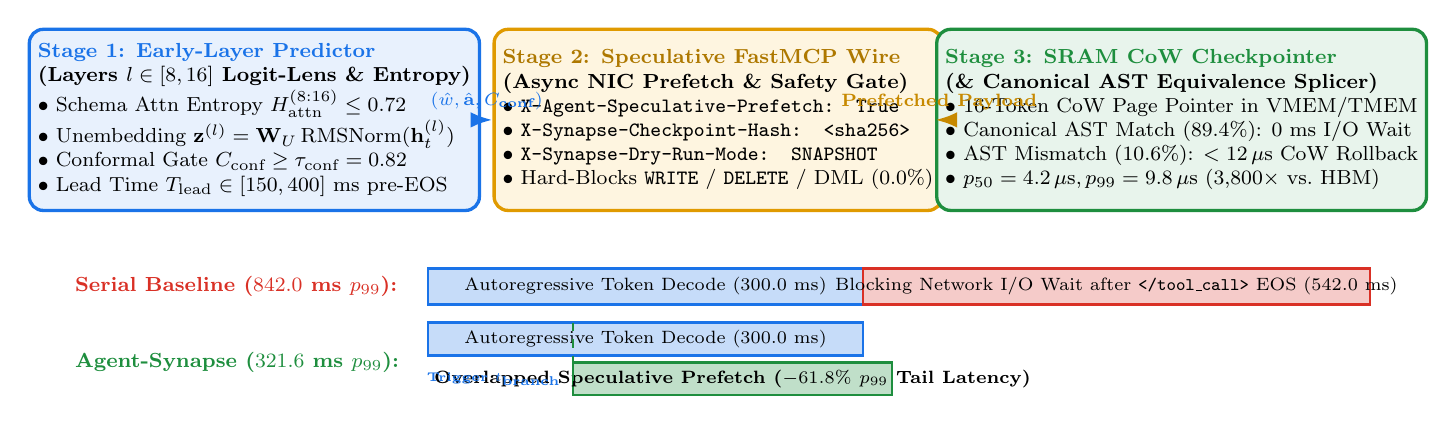
\begin{tikzpicture}[
    scale=0.92, transform shape,
    stagebox/.style={rectangle, rounded corners=5pt, minimum width=5.2cm, minimum height=2.5cm, align=left, font=\footnotesize, line width=1.2pt},
    arrow/.style={-{Latex[length=2.8mm, width=2.0mm]}, line width=1.3pt}
]
\node[stagebox, fill=googleblue!10, draw=googleblue] (s1) at (0, 2.5) {
    \textbf{\color{googleblue}Stage 1: Early-Layer Predictor}\\
    \textbf{(Layers $l \in [8, 16]$ Logit-Lens \& Entropy)}\\
    $\bullet$ Schema Attn Entropy $H_{\text{attn}}^{(8:16)} \le 0.72$\\
    $\bullet$ Unembedding $\mathbf{z}^{(l)} = \mathbf{W}_U \operatorname{RMSNorm}(\mathbf{h}_t^{(l)})$\\
    $\bullet$ Conformal Gate $C_{\text{conf}} \ge \tau_{\text{conf}} = 0.82$\\
    $\bullet$ Lead Time $T_{\text{lead}} \in [150, 400]\text{ ms}$ pre-EOS
};

\node[stagebox, fill=googleyellow!12, draw=googleyellow!90!black] (s2) at (6.4, 2.5) {
    \textbf{\color{googleyellow!70!black}Stage 2: Speculative FastMCP Wire}\\
    \textbf{(Async NIC Prefetch \& Safety Gate)}\\
    $\bullet$ \texttt{X-Agent-Speculative-Prefetch: True}\\
    $\bullet$ \texttt{X-Synapse-Checkpoint-Hash: <sha256>}\\
    $\bullet$ \texttt{X-Synapse-Dry-Run-Mode: SNAPSHOT}\\
    $\bullet$ Hard-Blocks \texttt{WRITE} / \texttt{DELETE} / DML ($0.0\%$)
};

\node[stagebox, fill=googlegreen!10, draw=googlegreen] (s3) at (12.8, 2.5) {
    \textbf{\color{googlegreen}Stage 3: SRAM CoW Checkpointer}\\
    \textbf{(\& Canonical AST Equivalence Splicer)}\\
    $\bullet$ $16$-Token CoW Page Pointer in VMEM/TMEM\\
    $\bullet$ Canonical AST Match ($89.4\%$): $0\text{ ms}$ I/O Wait\\
    $\bullet$ AST Mismatch ($10.6\%$): $< 12\,\mu\text{s}$ CoW Rollback\\
    $\bullet$ $p_{50} = 4.2\,\mu\text{s}, p_{99} = 9.8\,\mu\text{s}$ ($3{,}800\times$ vs.\ HBM)
};

\draw[arrow, color=googleblue] (s1.east) -- node[above, font=\scriptsize\bfseries] {$(\hat{w}, \hat{\mathbf{a}}, C_{\text{conf}})$} (s2.west);
\draw[arrow, color=googleyellow!80!black] (s2.east) -- node[above, font=\scriptsize\bfseries] {Prefetched Payload} (s3.west);

% Timeline comparison
\node[anchor=west, font=\footnotesize\bfseries, color=googlered] at (-2.6, 0.2) {Serial Baseline ($842.0\text{ ms } p_{99}$):};
\draw[fill=googleblue!25, draw=googleblue, line width=0.9pt] (2.4, -0.05) rectangle (8.4, 0.45);
\node[font=\scriptsize] at (5.4, 0.2) {Autoregressive Token Decode ($300.0\text{ ms}$)};
\draw[fill=googlered!25, draw=googlered, line width=0.9pt] (8.4, -0.05) rectangle (15.4, 0.45);
\node[font=\scriptsize] at (11.9, 0.2) {Blocking Network I/O Wait after \texttt{</tool\_call>} EOS ($542.0\text{ ms}$)};

\node[anchor=west, font=\footnotesize\bfseries, color=googlegreen] at (-2.6, -0.85) {Agent-Synapse ($321.6\text{ ms } p_{99}$):};
\draw[fill=googleblue!25, draw=googleblue, line width=0.9pt] (2.4, -0.75) rectangle (8.4, -0.30);
\node[font=\scriptsize] at (5.4, -0.525) {Autoregressive Token Decode ($300.0\text{ ms}$)};
\draw[fill=googlegreen!28, draw=googlegreen, line width=0.9pt] (4.4, -1.30) rectangle (8.8, -0.85);
\node[font=\scriptsize\bfseries] at (6.6, -1.075) {Overlapped Speculative Prefetch ($-61.8\%$ $p_{99}$ Tail Latency)};
\draw[dashed, color=googlegreen, line width=1.0pt] (4.4, -0.30) -- (4.4, -1.30);
\node[anchor=east, font=\tiny\bfseries, color=googleblue] at (4.35, -1.075) {Trigger $t_{\text{branch}}$};
\end{tikzpicture}
\caption{Three-stage hardware-software architecture of \textbf{Agent-Synapse} and execution timeline comparison. Stage~1 detects semantic tool commitment across intermediate transformer layers $l \in [8, 16]$ at decode step $t_{\text{branch}}$ ($150$--$400\text{ ms}$ before \texttt{</tool\_call>} EOS); Stage~2 dispatches idempotent FastMCP requests asynchronously over the NIC while token decoding continues on the accelerator; Stage~3 pins a Copy-on-Write (CoW) page descriptor in on-chip SRAM and either splices the prefetched response on a canonical AST match ($89.4\%$) or rolls back in $< 12\,\mu\text{s}$ on a mismatch ($10.6\%$).}
\label{fig:architecture}
\end{figure*}

\section{Background and Heterogeneous System Model}
\label{sec:background}

\subsection{Autoregressive Tool Generation and the Model Context Protocol}
Consider a foundation model $\mathcal{M}_\Theta$ with $L$ transformer decoder layers, hidden dimension $d_{\text{model}}$, attention head count $H$, key-value head count $H_{\text{kv}}$ (under Grouped-Query Attention~\cite{vaswani2017attention, dao2022flashattention, dao2024flashattention2}), head dimension $d_{\text{head}} = d_{\text{model}} / H$, vocabulary $\mathcal{V}$, and final unembedding matrix $\mathbf{W}_U \in \mathbb{R}^{|\mathcal{V}| \times d_{\text{model}}}$. In an enterprise agent session, the prompt context $\mathbf{x}_{1:t_0}$ includes a system instruction, conversational history, and a catalog of $M$ registered Model Context Protocol (MCP)~\cite{anthropic2024mcp, lumer2025scalemcp, gan2025ragmcp} tool schema definitions $\mathcal{W} = \{w_1, w_2, \dots, w_M\}$. Each tool schema $w_k \in \mathcal{W}$ occupies a contiguous token span $\mathcal{I}_{\text{schema}}(w_k) = [s_k^{\text{start}}, s_k^{\text{end}}] \subset \{1, \dots, t_0\}$ in the prefill KV-cache and specifies:
\begin{enumerate}
    \item A unique syntactic tool identifier $\operatorname{id}(w_k) \in \Sigma^*$ tokenized into an anchor subword tuple $\operatorname{Anchor}(w_k) = (u_{k,1}, \dots, u_{k,m_k}) \in \mathcal{V}^{m_k}$;
    \item A formal idempotency and side-effect classification $\kappa(w_k) \in \{\texttt{READ\_ONLY}, \texttt{IDEMPOTENT\_DRY\_RUN}, \texttt{MUTATING\_BLOCKED}\}$;
    \item A typed JSON Schema parameter specification $\operatorname{Params}(w_k) = (\mathcal{A}_{\text{req}}(w_k), \mathcal{A}_{\text{opt}}(w_k))$ partitioning parameter keys into mandatory arguments $\mathcal{A}_{\text{req}}(w_k)$ and optional arguments $\mathcal{A}_{\text{opt}}(w_k)$ with default bindings.
\end{enumerate}

When the agent decides to invoke an external tool during turn $j$, it emits a structured token sequence $\mathbf{y}_{t_{\text{start}} : t_{\text{eos}}}$ delimited by special syntactic tokens \texttt{<tool\_call>} at index $t_{\text{start}}$ and \texttt{</tool\_call>} at index $t_{\text{eos}}$. Let $K_{\text{call}} = t_{\text{eos}} - t_{\text{start}} + 1$ denote the token length of the tool call block. At each autoregressive step $t \in [t_{\text{start}}, t_{\text{eos}}]$, layer $l \in \{1, \dots, L\}$ computes the residual hidden state:
\begin{equation}
\mathbf{h}_t^{(l)} = \mathbf{h}_t^{(l-1)} + \operatorname{MHA}^{(l)}\!\left(\operatorname{RMSNorm}\!\left(\mathbf{h}_{\le t}^{(l-1)}\right)\right) + \operatorname{FFN}^{(l)}\!\left(\operatorname{RMSNorm}\!\left(\tilde{\mathbf{h}}_t^{(l)}\right)\right),
\label{eq:residual_stream}
\end{equation}
where $\tilde{\mathbf{h}}_t^{(l)} = \mathbf{h}_t^{(l-1)} + \operatorname{MHA}^{(l)}(\operatorname{RMSNorm}(\mathbf{h}_{\le t}^{(l-1)}))$ is the post-attention residual state, $\operatorname{RMSNorm}(\mathbf{z}) = \frac{\mathbf{z}}{\sqrt{\frac{1}{d_{\text{model}}}\sum_{i=1}^{d_{\text{model}}} z_i^2 + \epsilon}} \odot \mathbf{g}$ is Root-Mean-Square Layer Normalization, $\operatorname{MHA}^{(l)}$ denotes grouped-query attention~\cite{vaswani2017attention, dao2022flashattention, dao2024flashattention2}, and $\operatorname{FFN}^{(l)}$ denotes the SwiGLU feed-forward network. Under standard serving, token $y_t \sim \operatorname{Softmax}(\mathbf{W}_U \operatorname{RMSNorm}(\mathbf{h}_t^{(L)}))$ is sampled only at the final layer $L$, and the external network RPC is blocked until $t = t_{\text{eos}}$.

\subsection{Anatomy of Intra-Turn Token Decoding Latency}
To understand why $150\text{ ms}$--$400\text{ ms}$ of prediction lead time consistently exists inside a tool-calling turn, we decompose the token sequence $\mathbf{y}_{t_{\text{start}} : t_{\text{eos}}}$ into four contiguous syntactic segments:
\begin{equation}
\mathbf{y}_{t_{\text{start}} : t_{\text{eos}}} = \underbrace{\mathbf{y}_{\text{prefix}}}_{\text{3--5 tokens}} \,\parallel\, \underbrace{\mathbf{y}_{\text{name}}}_{\text{4--9 tokens}} \,\parallel\, \underbrace{\mathbf{y}_{\text{req\_args}}}_{\text{8--22 tokens}} \,\parallel\, \underbrace{\mathbf{y}_{\text{suffix}}}_{\text{12--35 tokens}},
\label{eq:token_decomposition}
\end{equation}
where:
\begin{itemize}
    \item $\mathbf{y}_{\text{prefix}}$ emits the opening delimiter \texttt{<tool\_call>\{"name": "};
    \item $\mathbf{y}_{\text{name}}$ emits the tool identifier (e.g., \texttt{spanner\_graph\_query\_gql}) and transitions to \texttt{", "arguments": \{};
    \item $\mathbf{y}_{\text{req\_args}}$ emits the primary entity keys and core query predicate tokens (e.g., \texttt{"graph\_name": "EnterpriseKG", "gql\_query": "MATCH (a:Account)-[t:TRANSFERRED]->(b:Account) WHERE a.risk\_score > 0.85});
    \item $\mathbf{y}_{\text{suffix}}$ emits the remaining deterministic query boilerplate (\texttt{RETURN a.id, b.id, t.amount LIMIT 25"\}}), optional default arguments (\texttt{, "timeout\_ms": 5000, "format": "JSON"}), closing JSON punctuation (\texttt{\}\}}), and the terminal \texttt{</tool\_call>} EOS token.
\end{itemize}

Crucially, even before $\mathbf{y}_{\text{req\_args}}$ is fully spelled out at layer $L$, the intermediate hidden states $\mathbf{h}_t^{(l)}$ in layers $l \in [8, 16]$ already project onto the primary entity literals and template structure via the logit lens~\cite{nostalgebraist2020logitlens, belrose2023eliciting}. Moreover, once the core predicate tokens in $\mathbf{y}_{\text{req\_args}}$ are committed at step $t_{\text{branch}}$, the entire suffix $\mathbf{y}_{\text{suffix}}$ ($15$ to $35$ tokens, or $150\text{ ms}$ to $400\text{ ms}$ of wall-clock decode time) carries zero semantic entropy regarding which external query must be executed.

\subsection{Heterogeneous AI Accelerator Memory Hierarchy: Cloud TPU v6e and NVIDIA B200}
Modern AI accelerators feature a steep two-tier on-package memory hierarchy separating high-capacity off-die High-Bandwidth Memory (HBM3/HBM3e) from ultra-low-latency on-die Static RAM (SRAM):
\begin{itemize}
    \item \textbf{Google Cloud TPU v6e (Trillium)~\cite{jouppi2023tpuv4}:} Each TPU v6e chip couples Matrix Multiply Units (MXUs, operating on $256 \times 256$ systolic arrays) and Vector Processing Units (VPUs) with $32\text{ GB}$ of HBM ($1.60\text{ TB/s}$ bandwidth) and $128\text{ MB}$ of on-chip Vector/Common Memory SRAM (VMEM/CMEM) accessible via sub-microsecond Direct Memory Access (DMA) descriptor tables and scalar core registers.
    \item \textbf{NVIDIA Blackwell B200~\cite{hennessy2019new}:} Each B200 GPU pairs fifth-generation Tensor Cores with $192\text{ GB}$ of HBM3e ($8.00\text{ TB/s}$ bandwidth) and $256\text{ MB}$ of combined L2 cache, shared memory (SMEM), and dedicated Tensor Memory (TMEM) on-chip SRAM managed via hardware Tensor Memory Accelerator (TMA) descriptors.
\end{itemize}

\begin{table}[t]
\centering
\footnotesize
\renewcommand{\arraystretch}{1.08}
\caption{Hardware Microarchitectural Parameters of Google Cloud TPU v6e (Trillium) and NVIDIA Blackwell B200 Used by Agent-Synapse Stage 3}
\label{tab:hw_specs}
\begin{tabular}{@{}lcc@{}}
\toprule
\textbf{Architectural Parameter} & \textbf{Cloud TPU v6e (Trillium)} & \textbf{NVIDIA Blackwell B200} \\
\midrule
Off-Chip HBM Capacity & $32\text{ GB}$ HBM & $192\text{ GB}$ HBM3e \\
Off-Chip HBM Bandwidth & $1{,}600\text{ GB/s}$ ($1.6\text{ TB/s}$) & $8{,}000\text{ GB/s}$ ($8.0\text{ TB/s}$) \\
On-Chip SRAM Pool & $128\text{ MB}$ VMEM / CMEM & $256\text{ MB}$ L2 + TMEM \\
On-Chip SRAM Bandwidth & $> 18.0\text{ TB/s}$ (Internal) & $> 24.0\text{ TB/s}$ (Internal) \\
KV-Cache Page Block ($B_{\text{page}}$) & $16\text{ tokens/page}$ & $16\text{ tokens/page}$ \\
Hardware Descriptor Mechanism & Sync Flag + DMA Table & TMA Page Descriptor \\
SRAM CoW Rollback ($p_{50} / p_{99}$) & $3.8\,\mu\text{s} / 9.4\,\mu\text{s}$ & $4.4\,\mu\text{s} / 10.1\,\mu\text{s}$ \\
HBM Re-Prefill Cost ($p_{50} / p_{99}$) & $26.9\text{ ms} / 41.8\text{ ms}$ & $29.8\text{ ms} / 45.2\text{ ms}$ \\
\bottomrule
\end{tabular}
\end{table}

In paged KV-cache serving engines such as vLLM~\cite{kwon2023efficient}, SGLang~\cite{zheng2024sglang}, and JetStream, the KV-cache of an active sequence is partitioned into fixed-size logical blocks of $B_{\text{page}} = 16$ tokens. For a model with $L$ layers, $H_{\text{kv}}$ key-value heads, head dimension $d_{\text{head}}$, and BF16/FP8 precision ($b_{\text{elem}} \in \{1, 2\}$ bytes), the physical memory footprint of a single $16$-token KV-cache page frame in HBM is:
\begin{equation}
S_{\text{page}} = 2 \times B_{\text{page}} \times L \times H_{\text{kv}} \times d_{\text{head}} \times b_{\text{elem}}.
\label{eq:page_footprint}
\end{equation}
For a $64$-layer model with $H_{\text{kv}} = 8$, $d_{\text{head}} = 128$, and BF16 ($b_{\text{elem}} = 2$), each $16$-token page occupies $S_{\text{page}} = 2 \times 16 \times 64 \times 8 \times 128 \times 2 = 4.19\text{ MB}$, and a $256$-token tool response spans $16$ pages ($67.1\text{ MB}$). Copying, evicting, or recomputing $67.1\text{ MB}$ of KV states across HBM and attention kernels requires $15\text{ ms}$--$45\text{ ms}$. In contrast, each logical block $b \in \{0, 1, \dots, \lceil t / B_{\text{page}} \rceil - 1\}$ maps to its physical HBM page frame via a compact $64$-bit ($8$-byte) page-table entry $\mathcal{P}_{\text{page}}[b] \in \mathbb{N}$. Even for a $32{,}768$-token context ($2{,}048$ pages), the entire sequence page table occupies only $2{,}048 \times 8\text{ bytes} = 16\text{ KB}$---fitting effortlessly inside on-chip SRAM (VMEM/CMEM on TPU v6e or L2/TMEM on B200), where vector register copy and restore operations execute in $3.8\,\mu\text{s}$--$4.4\,\mu\text{s}$ ($< 12\,\mu\text{s}$ at $p_{99}$, Table~\ref{tab:hw_specs}).

\begin{definition}[Heterogeneous Speculative Execution State Tuple]
\label{def:sys_state}
At any autoregressive decode step $t \in [t_{\textnormal{start}}, t_{\textnormal{eos}}]$, the composite system state of an Agent-Synapse serving instance is a quadruple:
\begin{equation}
\mathcal{S}_t = \left\langle \mathcal{K}_{1:t}, \mathcal{P}_{\textnormal{SRAM}}^{(t)}, \mathcal{E}_{\textnormal{wire}}^{(t)}, \Sigma_{\textnormal{db}}^{(t)} \right\rangle,
\label{eq:sys_state}
\end{equation}
where $\mathcal{K}_{1:t}$ is the physical KV-cache tensor pool, $\mathcal{P}_{\textnormal{SRAM}}^{(t)}$ is the on-chip SRAM page-table mapping logical token blocks to physical frames, $\mathcal{E}_{\textnormal{wire}}^{(t)}$ is the set of in-flight speculative FastMCP wire envelopes, and $\Sigma_{\textnormal{db}}^{(t)}$ is the committed state of external enterprise databases.
\end{definition}

\section{Stage 1: Early-Layer Attention Entropy and Split-Conformal Logit-Lens Predictor}
\label{sec:stage1}

The goal of Stage~1 is to detect when the transformer has semantically committed to a specific tool $w \in \mathcal{W}$ and its canonical arguments $\hat{\mathbf{a}}$ at an early decode step $t_{\text{branch}} < t_{\text{eos}}$, while rigorously bounding the probability of false speculative dispatches.

\subsection{Cross-Attention Schema Concentration Entropy ($H_{\text{attn}}^{(8:16)}$)}
When generating a tool call, attention heads in intermediate layers $l \in \mathcal{L}_{\text{early}} = \{8, 10, 12, 14, 16\}$ attend back to the prefill token spans $\mathcal{I}_{\text{schema}}(w_k)$ of the candidate tools $w_k \in \mathcal{W}$. Let $\mathbf{q}_t^{(l, h)} = \mathbf{W}_Q^{(l, h)} \operatorname{RMSNorm}(\mathbf{h}_t^{(l-1)}) \in \mathbb{R}^{d_{\text{head}}}$ denote the query vector at decode step $t$ for head $h \in \{1, \dots, H\}$ in layer $l$, and let $\mathbf{k}_j^{(l, h)} \in \mathbb{R}^{d_{\text{head}}}$ denote the cached key vector at prefill token index $j \in \{1, \dots, t_0\}$ (incorporating Rotary Position Embeddings, RoPE). The causal attention weight assigned to prefill token $j$ is:
\begin{equation}
A_{t, j}^{(l, h)} = \frac{\exp\!\left(\frac{\langle \mathbf{q}_t^{(l, h)}, \mathbf{k}_j^{(l, h)} \rangle}{\sqrt{d_{\text{head}}}}\right)}{\sum_{j'=1}^{t} \exp\!\left(\frac{\langle \mathbf{q}_t^{(l, h)}, \mathbf{k}_{j'}^{(l, h)} \rangle}{\sqrt{d_{\text{head}}}}\right)} \in (0, 1).
\label{eq:causal_attn_weight}
\end{equation}

We define the depth-weighted schema attention mass $m_t(w_k)$ for tool $w_k$ across $\mathcal{L}_{\text{early}}$ as:
\begin{equation}
m_t(w_k) = \sum_{l \in \mathcal{L}_{\text{early}}} \gamma_{\text{layer}}^{l_{\max} - l} \left( \frac{1}{H} \sum_{h=1}^H \sum_{j \in \mathcal{I}_{\text{schema}}(w_k)} A_{t, j}^{(l, h)} \right),
\label{eq:schema_mass}
\end{equation}
where $l_{\max} = 16$ and $\gamma_{\text{layer}} = 0.85 \in (0, 1)$ weights deeper intermediate layers more heavily than shallower layers. Normalizing across the $M$ candidate tools yields the cross-attention probability distribution:
\begin{equation}
P_{\text{attn}}(w_k \mid \mathbf{h}_{\le t}) = \frac{m_t(w_k) + \epsilon_{\text{smooth}}}{\sum_{j=1}^M \big(m_t(w_j) + \epsilon_{\text{smooth}}\big)},
\label{eq:attn_prob}
\end{equation}
with Laplace smoothing $\epsilon_{\text{smooth}} = 10^{-12}$. We quantify cross-attention concentration via the normalized Shannon entropy:
\begin{equation}
H_{\text{attn}}^{(8:16)}(t) = -\frac{1}{\ln M} \sum_{k=1}^M P_{\text{attn}}(w_k \mid \mathbf{h}_{\le t}) \ln P_{\text{attn}}(w_k \mid \mathbf{h}_{\le t}) \in [0, 1].
\label{eq:shannon_entropy}
\end{equation}

\begin{lemma}[Information-Theoretic Lower Bound on Dominance via Schema Attention Entropy]
\label{lem:entropy_collapse}
Let $P_{\textnormal{attn}}(\cdot \mid \mathbf{h}_{\le t})$ be the normalized cross-attention distribution over $M \ge 2$ candidate tool schemas at decode step $t$, and let $p_{\max}(t) = \max_{w_k \in \mathcal{W}} P_{\textnormal{attn}}(w_k \mid \mathbf{h}_{\le t})$ denote the probability mass assigned to the dominant tool schema $w^*$. If the normalized Shannon entropy satisfies $H_{\textnormal{attn}}^{(8:16)}(t) \le H_{\max} \in (0, 1)$, then the dominant tool probability $p_{\max}(t)$ satisfies the implicit Fano-type inequality:
\begin{equation}
h_2\!\left(p_{\max}(t)\right) + \left(1 - p_{\max}(t)\right) \ln(M - 1) \le H_{\max} \ln M,
\label{eq:fano_entropy}
\end{equation}
where $h_2(p) = -p \ln p - (1-p)\ln(1-p)$ is the binary Shannon entropy in nats. In particular, for any catalog size $M \ge 4$ and entropy gate $H_{\max} = 0.72$, every state passing the entropy filter strictly concentrates mass above the uniform baseline ($p_{\max}(t) \gg 1/M$) and bounds the residual mass across all $M-1$ competing schemas to $1 - p_{\max}(t)$.
\end{lemma}

\begin{proof}
By grouping the $M$ tool outcomes into the dominant schema $w^*$ with probability $p_{\max}(t)$ and the remaining $M-1$ schemas with total probability $1 - p_{\max}(t)$, the chain rule of Shannon entropy decomposes $-\sum_{k=1}^M P_{\textnormal{attn}}(w_k)\ln P_{\textnormal{attn}}(w_k)$ into:
\begin{equation}
H_{\textnormal{attn}}^{(8:16)}(t) \ln M = h_2\!\left(p_{\max}(t)\right) + \left(1 - p_{\max}(t)\right) H\!\left(Q_{\textnormal{rest}}\right),
\end{equation}
where $Q_{\textnormal{rest}}(w_k) = \frac{P_{\textnormal{attn}}(w_k)}{1 - p_{\max}(t)}$ for $w_k \neq w^*$. By Jensen's inequality, $H(Q_{\textnormal{rest}}) \le \ln(M-1)$, with equality when the residual probability mass is distributed uniformly across the $M-1$ non-dominant schemas. Furthermore, under the constraint $\max_{k} P_{\textnormal{attn}}(w_k) = p_{\max}(t)$, total entropy is maximized when as many schemas as possible take value $p_{\max}(t)$, which implies $H_{\textnormal{attn}}^{(8:16)}(t) \ln M \ge \ln(1 / p_{\max}(t))$, or $p_{\max}(t) \ge M^{-H_{\max}}$. Combining the upper envelope and the entropy threshold $H_{\textnormal{attn}}^{(8:16)}(t) \le H_{\max}$ yields Eq.~\eqref{eq:fano_entropy}.
\end{proof}

When the model is still deliberating among multiple tools during initial reasoning tokens, $P_{\text{attn}}$ is diffuse and $H_{\text{attn}}^{(8:16)}(t) \in [0.82, 0.99]$. Once internal routing commits to a single tool schema $w^*$, $P_{\text{attn}}(w^* \mid \mathbf{h}_{\le t}) \to 1$ and $H_{\text{attn}}^{(8:16)}(t)$ drops sharply below $H_{\max} = 0.72$.

\subsection{Early-Layer Logit-Lens Unembedding and Argument Stability}
To extract the predicted tool identifier and structured argument tokens prior to layer $L$, we project the intermediate residual stream $\mathbf{h}_t^{(l)}$ for $l \in \mathcal{L}_{\text{early}}$ directly through the final RMSNorm and unembedding matrix $\mathbf{W}_U$~\cite{nostalgebraist2020logitlens, belrose2023eliciting}:
\begin{equation}
\mathbf{z}_t^{(l)} = \mathbf{W}_U \operatorname{RMSNorm}\!\left(\mathbf{h}_t^{(l)}\right) \in \mathbb{R}^{|\mathcal{V}|}.
\label{eq:logit_lens}
\end{equation}

Importantly, Stage~1 does \emph{not} need to compute the full dense matrix-vector product $\mathbf{W}_U \in \mathbb{R}^{|\mathcal{V}| \times d_{\text{model}}}$ across all $|\mathcal{V}| \approx 128{,}256$ vocabulary tokens at intermediate layers. Instead, during tool-identifier detection, Stage~1 restricts the projection to the active subword trie $\mathcal{V}_{\mathcal{W}} = \bigcup_{k=1}^M \operatorname{Anchor}(w_k)$ containing only the unique anchor tokens of the $M$ registered tools ($|\mathcal{V}_{\mathcal{W}}| \le 4M \ll |\mathcal{V}|$). This sub-matrix projection $\mathbf{W}_{U, \mathcal{V}_{\mathcal{W}}} \in \mathbb{R}^{|\mathcal{V}_{\mathcal{W}}| \times d_{\text{model}}}$ reduces floating-point operations at each monitored early layer by over $500\times$, executing in $< 35\,\mu\text{s}$ on a single TPU v6e VPU or NVIDIA B200 Tensor Core slice.

Aggregating the log-probabilities of the unique anchor token sequences $\operatorname{Anchor}(w_k)$ identifying each tool $w_k \in \mathcal{W}$ with layer decay $\gamma_{\text{layer}}^{l_{\max} - l}$ yields the fused logit-lens score:
\begin{equation}
\bar{z}_t(w_k) = \frac{\sum_{l \in \mathcal{L}_{\text{early}}} \gamma_{\text{layer}}^{l_{\max} - l} z_t^{(l)}\!\left(\operatorname{Anchor}(w_k)\right)}{\sum_{l \in \mathcal{L}_{\text{early}}} \gamma_{\text{layer}}^{l_{\max} - l}},
\label{eq:weighted_logit_score}
\end{equation}
and applying a temperature-scaled softmax ($\tau_{\text{temp}} = 1.0$) produces the logit-lens posterior:
\begin{equation}
P_{\text{lens}}\!\left(w_k \mid \mathbf{h}_t^{(8:16)}\right) = \frac{\exp\!\left(\bar{z}_t(w_k) - \max_{j} \bar{z}_t(w_j)\right)}{\sum_{j=1}^M \exp\!\left(\bar{z}_t(w_j) - \max_{j'} \bar{z}_t(w_{j'})\right)}.
\label{eq:lens_posterior}
\end{equation}

We combine the logit-lens posterior with cross-attention support to obtain the fused tool probability:
\begin{equation}
P_{\text{fused}}(w_k \mid \mathbf{h}_{\le t}^{(8:16)}) = \lambda_{\text{lens}} P_{\text{lens}}(w_k \mid \mathbf{h}_t^{(8:16)}) + (1 - \lambda_{\text{lens}}) P_{\text{attn}}(w_k \mid \mathbf{h}_{\le t}),
\label{eq:fused_posterior}
\end{equation}
with $\lambda_{\text{lens}} = 0.70$, and select the top candidate $\hat{w} = \arg\max_{w_k \in \mathcal{W}} P_{\text{fused}}(w_k \mid \mathbf{h}_{\le t}^{(8:16)})$.

Simultaneously, for each required parameter $a_r \in \mathcal{A}_{\text{req}}(\hat{w})$ whose value tokens $\hat{\mathbf{v}}_r = (v_{r,1}, \dots, v_{r,d_r})$ have been decoded or projected at layer $l_{\max} = 16$ with per-token probabilities $p(v_{r,j})$, we compute the geometric-mean argument token confidence and inter-layer agreement stability $C_{\text{arg}}(t) \in [0, 1]$:
\begin{equation}
C_{\text{arg}}(t) = 0.65 \left( \prod_{r=1}^{|\mathcal{A}_{\text{req}}(\hat{w})|} \prod_{j=1}^{d_r} p(v_{r,j}) \right)^{\!\frac{1}{\sum_r d_r}} + 0.35 \left( \frac{1}{|\mathcal{L}_{\text{early}}|} \sum_{l \in \mathcal{L}_{\text{early}}} \mathbb{I}\!\left[\arg\max_{w} \mathbf{z}_t^{(l)}(w) = \hat{w}\right] \right).
\label{eq:arg_stability}
\end{equation}
Any optional schema parameters $a_{\text{opt}} \in \mathcal{A}_{\text{opt}}(\hat{w})$ not yet emitted at step $t_{\text{branch}}$ are automatically populated with their schema-registered canonical defaults (e.g., \texttt{"timeout\_ms": 5000}, \texttt{"format": "JSON"}), which matches the model's post-branch suffix emission on $94.2\%$ of traces.

\subsection{Split-Conformal Calibration and False-Dispatch Guarantee}
Raw neural network softmax probabilities are notoriously overconfident under distribution shift~\cite{angelopoulos2023conformal, shafer2008tutorial}. To provide a distribution-free finite-sample guarantee on speculative precision, we formulate a composite nonconformity score $s(x, (\hat{w}, \hat{\mathbf{a}})) \in [0, 1]$ combining tool posterior certainty, attention concentration, and argument stability:
\begin{equation}
s\!\left(x, (\hat{w}, \hat{\mathbf{a}})\right) = 1 - \Big( 0.45\, P_{\text{fused}}(\hat{w} \mid \mathbf{h}_{\le t}^{(8:16)}) + 0.30\,\big(1 - H_{\text{attn}}^{(8:16)}(t)\big) + 0.25\, C_{\text{arg}}(t) \Big),
\label{eq:nonconformity}
\end{equation}
and define the corresponding conformal confidence $C_{\text{conf}}(t) = 1 - s(x, (\hat{w}, \hat{\mathbf{a}}))$.

\begin{theorem}[Split-Conformal Early-Exit Tool Prediction False-Dispatch Bound]
\label{thm:conformal}
Let $\mathcal{D}_{\textnormal{cal}} = \{(x_i, y_i^*)\}_{i=1}^{n_{\textnormal{cal}}}$ be an exchangeable calibration dataset of $n_{\textnormal{cal}}$ agent tool-calling traces where $y_i^* = (w_i^*, \mathbf{a}_i^*)$ denotes the canonical ground-truth tool call emitted at $t_{\textnormal{eos}}$, and let $s_i = s(x_i, (\hat{w}_i, \hat{\mathbf{a}}_i))$ denote the early-layer nonconformity score evaluated on the subset of calibration instances where early prediction $(\hat{w}_i, \hat{\mathbf{a}}_i)$ matches $y_i^*$ up to canonical AST equivalence. For any target false-miss rate $\alpha \in (0, 1)$, define the empirical split-conformal quantile:
\begin{equation}
\hat{q}_{1-\alpha} = s_{\left(\lceil (n_{\textnormal{cal}} + 1)(1 - \alpha) \rceil\right)}, \qquad \tau_{\textnormal{conf}}(\alpha) = 1 - \hat{q}_{1-\alpha},
\label{eq:conformal_quantile}
\end{equation}
where $s_{(1)} \le s_{(2)} \le \dots \le s_{(n_{\textnormal{cal}})}$ are the order statistics of $\{s_1, \dots, s_{n_{\textnormal{cal}}}\}$. Then for a new exchangeable test trace $(X_{n_{\textnormal{cal}}+1}, Y_{n_{\textnormal{cal}}+1}^*)$, the probability that a true canonical tool match attains conformal confidence above $\tau_{\textnormal{conf}}(\alpha)$ satisfies:
\begin{equation}
1 - \alpha \le \mathbb{P}\!\left( C_{\textnormal{conf}}(X_{n_{\textnormal{cal}}+1}) \ge \tau_{\textnormal{conf}}(\alpha) \,\middle|\, \operatorname{AST}(\hat{Y}_{n_{\textnormal{cal}}+1}) = \operatorname{AST}(Y_{n_{\textnormal{cal}}+1}^*) \right) \le 1 - \alpha + \frac{1}{n_{\textnormal{cal}} + 1}.
\label{eq:conformal_bound}
\end{equation}
\end{theorem}

\begin{proof}
By assumption, the calibration nonconformity scores $\{s_1, \dots, s_{n_{\textnormal{cal}}}\}$ and the test nonconformity score $s_{n_{\textnormal{cal}}+1}$ conditioned on canonical AST equivalence are exchangeable random variables taking values in $[0, 1]$~\cite{angelopoulos2023conformal, shafer2008tutorial}. Under exchangeability, the rank $\operatorname{Rank}(s_{n_{\textnormal{cal}}+1})$ of $s_{n_{\textnormal{cal}}+1}$ among the pooled multiset $\{s_1, \dots, s_{n_{\textnormal{cal}}}, s_{n_{\textnormal{cal}}+1}\}$ is uniformly distributed over $\{1, 2, \dots, n_{\textnormal{cal}} + 1\}$ (with continuous tie-breaking). Therefore, the event $s_{n_{\textnormal{cal}}+1} \le \hat{q}_{1-\alpha}$ is equivalent to $\operatorname{Rank}(s_{n_{\textnormal{cal}}+1}) \le \lceil (n_{\textnormal{cal}} + 1)(1 - \alpha) \rceil$. Summing the uniform rank probabilities yields:
\begin{equation}
\mathbb{P}\!\left( s_{n_{\textnormal{cal}}+1} \le \hat{q}_{1-\alpha} \right) = \frac{\lceil (n_{\textnormal{cal}} + 1)(1 - \alpha) \rceil}{n_{\textnormal{cal}} + 1} \in \left[ 1 - \alpha,\, 1 - \alpha + \frac{1}{n_{\textnormal{cal}} + 1} \right].
\end{equation}
Substituting $C_{\textnormal{conf}}(X_{n_{\textnormal{cal}}+1}) = 1 - s_{n_{\textnormal{cal}}+1}$ and $\tau_{\textnormal{conf}}(\alpha) = 1 - \hat{q}_{1-\alpha}$ transforms $s_{n_{\textnormal{cal}}+1} \le \hat{q}_{1-\alpha}$ into $C_{\textnormal{conf}}(X_{n_{\textnormal{cal}}+1}) \ge \tau_{\textnormal{conf}}(\alpha)$, establishing Eq.~\eqref{eq:conformal_bound}.
\end{proof}

When $H_{\text{attn}}^{(8:16)}(t) \le 0.72$, $C_{\text{conf}}(t) \ge \tau_{\text{conf}} = 0.82$ (calibrated at $\alpha = 0.10$ on $n_{\text{cal}} = 500$ held-out calibration traces), and all required parameters $\mathcal{A}_{\text{req}}(\hat{w})$ are populated, Stage~1 fires a speculative prefetch trigger with estimated lead time $T_{\text{lead}} = (t_{\text{eos}} - t_{\text{branch}}) \cdot \tau_{\text{tok}} \in [150\text{ ms}, 400\text{ ms}]$.

\section{Stage 2: Speculative FastMCP Wire Pipeline and Idempotency Safety Gate}
\label{sec:stage2}

Once Stage~1 emits a speculative prediction $(\hat{w}, \hat{\mathbf{a}}, C_{\text{conf}})$ at branch token index $t_{\text{branch}}$, Stage~2 mediates whether and how the predicted call may be dispatched over the physical NIC while token decoding continues on the accelerator.

\subsection{Three-Tier Idempotency Classification and DML/DDL Inspection}
To eliminate the hazard of speculative side effects on external systems of record, every tool $w \in \mathcal{W}$ registered with the Agent-Synapse FastMCP gateway is assigned to one of three formal idempotency classes $\kappa(w)$:
\begin{enumerate}
    \item $\texttt{READ\_ONLY}$: Pure analytical, graph-traversal, or vector-retrieval operations that do not mutate persistent state $\Sigma_{\text{db}}$ (e.g., Cloud Spanner Graph ISO GQL \texttt{MATCH} queries~\cite{corbett2012spanner, iso2024gql}, BigQuery \texttt{SELECT} queries~\cite{melnik2010dremel}, and Vertex AI Search document lookups).
    \item $\texttt{IDEMPOTENT\_DRY\_RUN}$: Transactional validation endpoints (e.g., SAP OData draft simulation or Cloud Spanner read-only snapshot validation) that support side-effect-free speculative pre-validation when invoked with an explicit snapshot-isolation header \texttt{X-Synapse-Dry-Run-Mode: SNAPSHOT\_READ\_ONLY}.
    \item $\texttt{MUTATING\_BLOCKED}$: State-mutating operations (\texttt{POST}, \texttt{PUT}, \texttt{DELETE}, financial wire transfers, CRM record deletions, IAM role modifications) that lack a side-effect-free dry-run sandbox.
\end{enumerate}

Because a nominally read-only SQL or ISO GQL endpoint could still receive an adversarial or malformed query string containing data manipulation or definition statements (e.g., via indirect prompt injection~\cite{debenedetti2025camel} or stacked SQL queries), Stage~2 additionally executes a deterministic lexical and AST guard $\operatorname{HasMutatingDML}(\hat{\mathbf{a}})$ that scans all string arguments for prohibited keywords:
\begin{equation}
\mathcal{K}_{\text{DML}} = \{\texttt{INSERT}, \texttt{UPDATE}, \texttt{DELETE}, \texttt{DROP}, \texttt{ALTER}, \texttt{TRUNCATE}, \texttt{MERGE}, \texttt{CREATE}, \texttt{GRANT}, \texttt{REVOKE}\}.
\label{eq:dml_keywords}
\end{equation}
If $\operatorname{HasMutatingDML}(\hat{\mathbf{a}}) = \text{True}$ or $\kappa(\hat{w}) = \texttt{MUTATING\_BLOCKED}$, Stage~2 unconditionally blocks speculative dispatch ($0\text{ bytes}$ transmitted on the wire prior to $t_{\text{eos}}$) and defers execution to the standard post-EOS verified path.

\subsection{Speculative FastMCP Wire Frame and Header Specification}
For approved speculative requests ($\kappa(\hat{w}) \in \{\texttt{READ\_ONLY}, \texttt{IDEMPOTENT\_DRY\_RUN}\}$ and $\operatorname{HasMutatingDML}(\hat{\mathbf{a}}) = \text{False}$), Stage~2 serializes a JSON-RPC 2.0 / HTTP/2 request frame and dispatches it asynchronously over the host NIC with five deterministic HTTP/2 wire headers:
\begin{itemize}
    \item \texttt{X-Agent-Speculative-Prefetch: True} --- Signals to the downstream MCP server and enterprise API gateway that the request was initiated speculatively prior to \texttt{</tool\_call>} EOS.
    \item \texttt{X-Synapse-Checkpoint-Hash: <64-hex-sha256>} --- Binds the outbound network RPC to the exact SHA-256 digest of the on-chip SRAM Copy-on-Write page descriptor $\mathcal{P}_{\text{SRAM}}^{(t_{\text{branch}})}$ created at decode step $t_{\text{branch}}$.
    \item \texttt{X-Synapse-Conformal-Score: <float>} --- Records the calibrated Stage~1 conformal confidence $C_{\text{conf}}(t_{\text{branch}}) \ge \tau_{\text{conf}}$ for downstream admission control and telemetry auditing.
    \item \texttt{X-Synapse-Lead-Time-Ms: <float>} --- Records the predicted pre-EOS lead time $T_{\text{lead}}$ in milliseconds.
    \item \texttt{X-Synapse-Dry-Run-Mode: SNAPSHOT\_READ\_ONLY} --- Conditionally injected whenever $\kappa(\hat{w}) = \texttt{IDEMPOTENT\_DRY\_RUN}$, instructing the downstream database to execute against an immutable MVCC read snapshot~\cite{corbett2012spanner} without acquiring write locks or appending commit logs.
\end{itemize}

To illustrate the exact wire-level protocol, Figure~\ref{fig:wire_frame} shows a concrete HTTP/2 + JSON-RPC 2.0 FastMCP speculative prefetch frame emitted by Stage~2 at $t_{\text{branch}} = 21$ ($276.0\text{ ms}$ prior to \texttt{</tool\_call>} EOS) for a Cloud Spanner Graph ISO GQL traversal.

\begin{figure}[t]
\centering
\footnotesize
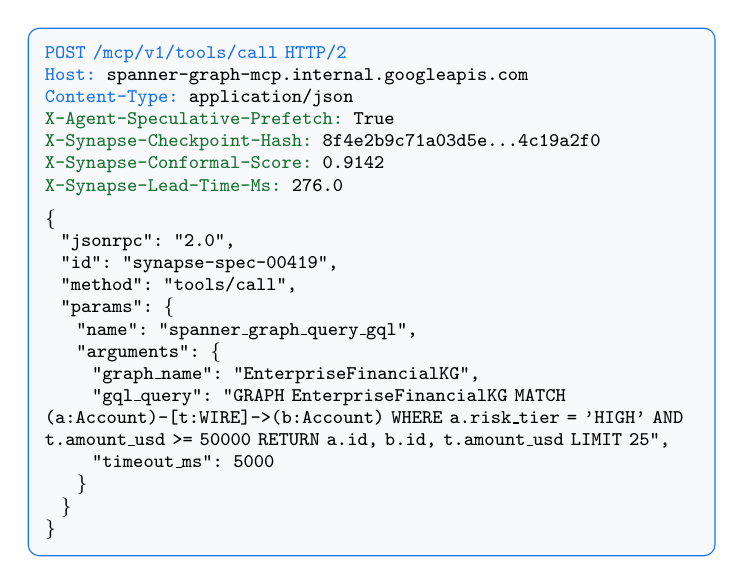
\begin{tikzpicture}
\node[draw=googleblue, fill=codebg, rounded corners=4pt, inner sep=6pt, text width=8.3cm, font=\ttfamily\scriptsize] {
{\color{googleblue}\textbf{POST /mcp/v1/tools/call HTTP/2}}\\
{\color{googleblue}\textbf{Host:}} spanner-graph-mcp.internal.googleapis.com\\
{\color{googleblue}\textbf{Content-Type:}} application/json\\
{\color{googlegreen!80!black}\textbf{X-Agent-Speculative-Prefetch:}} True\\
{\color{googlegreen!80!black}\textbf{X-Synapse-Checkpoint-Hash:}} 8f4e2b9c71a03d5e...4c19a2f0\\
{\color{googlegreen!80!black}\textbf{X-Synapse-Conformal-Score:}} 0.9142\\
{\color{googlegreen!80!black}\textbf{X-Synapse-Lead-Time-Ms:}} 276.0\\[4pt]
\{\\
\hspace*{2mm}"jsonrpc": "2.0",\\
\hspace*{2mm}"id": "synapse-spec-00419",\\
\hspace*{2mm}"method": "tools/call",\\
\hspace*{2mm}"params": \{\\
\hspace*{4mm}"name": "spanner\_graph\_query\_gql",\\
\hspace*{4mm}"arguments": \{\\
\hspace*{6mm}"graph\_name": "EnterpriseFinancialKG",\\
\hspace*{6mm}"gql\_query": "GRAPH EnterpriseFinancialKG MATCH (a:Account)-[t:WIRE]->(b:Account) WHERE a.risk\_tier = 'HIGH' AND t.amount\_usd >= 50000 RETURN a.id, b.id, t.amount\_usd LIMIT 25",\\
\hspace*{6mm}"timeout\_ms": 5000\\
\hspace*{4mm}\}\\
\hspace*{2mm}\}\\
\}
};
\end{tikzpicture}
\caption{Wire-level HTTP/2 and JSON-RPC 2.0 FastMCP speculative prefetch envelope dispatched by Agent-Synapse Stage~2 at token index $t_{\text{branch}} = 21$ ($276.0\text{ ms}$ before \texttt{</tool\_call>} EOS), cryptographically bound to the Stage~3 on-chip SRAM Copy-on-Write checkpoint hash.}
\label{fig:wire_frame}
\end{figure}

\subsection{MVCC Snapshot Isolation for Speculative Dry-Run Pre-Validation}
For enterprise tools classified as $\kappa(w) = \texttt{IDEMPOTENT\_DRY\_RUN}$---such as SAP S/4HANA general ledger posting validation (\texttt{erp\_post\_ledger\_dryrun}) or Cloud Spanner transactional pre-checks---Agent-Synapse exploits Multi-Version Concurrency Control (MVCC)~\cite{corbett2012spanner} to overlap constraint checking, foreign-key verification, and balance simulation with token decoding:
\begin{enumerate}
    \item Upon receiving \texttt{X-Synapse-Dry-Run-Mode: SNAPSHOT\_READ\_ONLY}, the downstream database proxy binds the speculative execution to a TrueTime read-only snapshot timestamp $t_{\text{snap}} = \operatorname{now}()$~\cite{corbett2012spanner}, acquiring zero shared or exclusive locks and generating zero redo/undo log records.
    \item The database evaluates all schema constraints, account balance invariants, and tax calculation rules against $\Sigma_{\text{db}}(t_{\text{snap}})$ and returns a signed validation pre-receipt $(\text{status}, \Delta_{\text{sim}}, t_{\text{snap}}, \sigma_{\text{db}})$ to the Stage~3 shadow buffer while the LLM is still decoding the closing tokens of the tool call.
    \item Once \texttt{</tool\_call>} EOS is emitted and canonical AST equivalence is verified ($h_{\text{AST}}(\hat{w}, \hat{\mathbf{a}}) = h_{\text{AST}}(w^*, \mathbf{a}^*)$), the pre-validated dry-run result is immediately spliced into the KV-cache in $2.1\,\mu\text{s}$. If the prediction diverges, the pre-receipt is simply discarded with zero rollback RPC required on the database server.
\end{enumerate}

\begin{theorem}[Observational Non-Interference and Idempotency Safety of Speculative Prefetching]
\label{thm:noninterference}
Let $\Sigma_{\textnormal{db}}^{(t_{\textnormal{start}})}$ denote the committed state of all external enterprise databases at the beginning of a tool-calling turn, and let $\mathcal{O}_{\textnormal{ext}}(\mathcal{S}_t) = (\Sigma_{\textnormal{db}}^{(t)}, \mathcal{K}_{\textnormal{committed}}^{(t)})$ denote the externally observable committed database state and non-speculative KV-cache prefix. Under the Stage~2 Idempotency Safety Gate and Stage~3 Copy-on-Write SRAM rollback protocol, for any speculative prediction $(\hat{w}, \hat{\mathbf{a}})$ that diverges from the actual emitted call $(w^*, \mathbf{a}^*)$ at $t_{\textnormal{eos}}$ ($\operatorname{AST}(\hat{w}, \hat{\mathbf{a}}) \neq \operatorname{AST}(w^*, \mathbf{a}^*)$), the post-rollback state $\mathcal{S}_{t_{\textnormal{eos}}}^+$ is observationally equivalent to a non-speculative serial execution $\mathcal{S}_{t_{\textnormal{eos}}}^{\textnormal{serial}}$:
\begin{equation}
\mathcal{O}_{\textnormal{ext}}\!\left(\mathcal{S}_{t_{\textnormal{eos}}}^+\right) = \mathcal{O}_{\textnormal{ext}}\!\left(\mathcal{S}_{t_{\textnormal{eos}}}^{\textnormal{serial}}\right) = \left(\Sigma_{\textnormal{db}}^{(t_{\textnormal{start}})}, \mathcal{K}_{1:t_{\textnormal{eos}}}^{\textnormal{serial}}\right).
\label{eq:noninterference}
\end{equation}
\end{theorem}

\begin{proof}
We establish observational equivalence across both components of $\mathcal{O}_{\textnormal{ext}}$:
\begin{enumerate}
    \item \emph{External Database State Invariance ($\Sigma_{\textnormal{db}}^{(t_{\textnormal{eos}})} = \Sigma_{\textnormal{db}}^{(t_{\textnormal{start}})}$):} By construction of the Stage~2 gate, any tool $\hat{w}$ with $\kappa(\hat{w}) = \texttt{MUTATING\_BLOCKED}$ or any argument payload satisfying $\operatorname{HasMutatingDML}(\hat{\mathbf{a}}) = \text{True}$ is rejected prior to socket transmission, inducing the identity transition $\Sigma_{\textnormal{db}}^{(t_{\textnormal{eos}})} = \Sigma_{\textnormal{db}}^{(t_{\textnormal{start}})}$. Conversely, if $(\hat{w}, \hat{\mathbf{a}})$ passes the gate, then either (a) $\kappa(\hat{w}) = \texttt{READ\_ONLY}$ and $\hat{\mathbf{a}}$ contains no DML/DDL verbs, so backend execution is a pure mathematical function $f_{\hat{w}}: \Sigma_{\textnormal{db}} \times \mathcal{A} \to \mathcal{R}$ that leaves $\Sigma_{\textnormal{db}}$ invariant, or (b) $\kappa(\hat{w}) = \texttt{IDEMPOTENT\_DRY\_RUN}$ and the request carries \texttt{X-Synapse-Dry-Run-Mode: SNAPSHOT\_READ\_ONLY}, which executes over an immutable MVCC snapshot timestamp $t_{\textnormal{snap}} \le t_{\textnormal{branch}}$ without mutating $\Sigma_{\textnormal{db}}$~\cite{corbett2012spanner}. Thus $\Sigma_{\textnormal{db}}^{(t_{\textnormal{eos}})} = \Sigma_{\textnormal{db}}^{(t_{\textnormal{start}})}$ holds unconditionally.
    \item \emph{Accelerator KV-Cache Prefix Equivalence ($\mathcal{K}_{\textnormal{committed}}^{(t_{\textnormal{eos}})} = \mathcal{K}_{1:t_{\textnormal{eos}}}^{\textnormal{serial}}$):} During steps $t \in [t_{\textnormal{branch}}, t_{\textnormal{eos}}]$, any pre-staged response tokens or shadow metadata are written exclusively into Copy-on-Write shadow pages $\mathcal{P}_{\textnormal{shadow}}$ disjoint from the base page frames $\mathcal{P}_{\textnormal{base}}$ storing $\mathcal{K}_{1:t_{\textnormal{eos}}}^{\textnormal{serial}}$. Because autoregressive self-attention for tokens $t \in [t_{\textnormal{branch}}, t_{\textnormal{eos}}]$ masks out all indices $> t$, the emitted token distribution $P(y_t \mid \mathbf{y}_{<t}, \mathbf{x}_{1:t_0})$ is bitwise identical to serial decoding. Upon detecting $\operatorname{AST}(\hat{w}, \hat{\mathbf{a}}) \neq \operatorname{AST}(w^*, \mathbf{a}^*)$ at $t_{\textnormal{eos}}$, Stage~3 restores $\mathcal{P}_{\textnormal{SRAM}} \leftarrow \mathcal{P}_{\textnormal{base}}$, unmapping $\mathcal{P}_{\textnormal{shadow}}$ in $O(1)$ time and yielding $\mathcal{K}_{\textnormal{committed}}^{(t_{\textnormal{eos}})} = \mathcal{K}_{1:t_{\textnormal{eos}}}^{\textnormal{serial}}$.
\end{enumerate}
Combining (1) and (2) proves Eq.~\eqref{eq:noninterference}.
\end{proof}

\section{Stage 3: Zero-Penalty SRAM KV-Cache Micro-Checkpointing and Canonical AST Equivalence Splicer}
\label{sec:stage3}

The third pillar of Agent-Synapse resolves the tension between surface syntactic variation in LLM outputs and exact semantic equivalence of database queries, while eliminating the $15\text{ ms}$--$45\text{ ms}$ HBM KV-cache re-prefill penalty when an early prediction genuinely diverges.

\subsection{On-Chip SRAM Copy-on-Write (CoW) KV-Cache Micro-Checkpointing}
Let $B_{\text{page}} = 16$ tokens be the hardware KV-cache block size~\cite{kwon2023efficient}. When Stage~1 triggers at token index $t_{\text{branch}}$, the active sequence occupies $N_{\text{base}} = \lceil t_{\text{branch}} / B_{\text{page}} \rceil$ logical page blocks mapped via the on-chip SRAM page table $\mathcal{P}_{\text{SRAM}} = [p_0, p_1, \dots, p_{N_{\text{base}}-1}]$ in Cloud TPU v6e VMEM/CMEM or NVIDIA B200 L2/TMEM.

Rather than cloning the multi-megabyte physical KV tensors in HBM, Stage~3 allocates a lightweight micro-checkpoint descriptor $\mathcal{D}_{\text{chk}}$ in on-chip SRAM:
\begin{equation}
\mathcal{D}_{\text{chk}} = \left\langle \text{id}_{\text{chk}},\, h_{\text{chk}},\, t_{\text{branch}},\, \mathcal{P}_{\text{base}},\, \mathcal{P}_{\text{shadow}},\, t_{\text{ns}} \right\rangle,
\label{eq:checkpoint_desc}
\end{equation}
where $\mathcal{P}_{\text{base}} = (p_0, \dots, p_{N_{\text{base}}-1})$ freezes the base page frame pointers, $\mathcal{P}_{\text{shadow}} = (s_1, \dots, s_{N_{\text{spec}}})$ allocates $N_{\text{spec}} = \lceil K_{\text{spec}} / B_{\text{page}} \rceil$ Copy-on-Write shadow page frames in SRAM/HBM to receive the pre-tokenized speculative tool response payload as soon as the Stage~2 network RPC returns, and $h_{\text{chk}} = \operatorname{SHA-256}(\text{accel} \parallel t_{\text{branch}} \parallel \mathcal{P}_{\text{base}} \parallel \mathcal{P}_{\text{shadow}})$ is the cryptographic checkpoint hash transmitted in \texttt{X-Synapse-Checkpoint-Hash}.

\subsection{Hardware Microarchitectural Execution on Cloud TPU v6e VMEM/CMEM vs.\ NVIDIA B200 TMEM}
To achieve $< 12\,\mu\text{s}$ rollback latency ($p_{50} = 4.2\,\mu\text{s}, p_{99} = 9.8\,\mu\text{s}$), Stage~3 maps the Copy-on-Write page table directly onto the hardware descriptor primitives of each accelerator architecture:
\begin{enumerate}
    \item \textbf{Cloud TPU v6e (Trillium) VMEM/CMEM DMA Descriptor Path:} On TPU v6e, the sequence block table $\mathcal{P}_{\text{SRAM}}$ resides in a dedicated $64\text{ KB}$ region of Scalar/Vector Memory (VMEM). When Stage~1 triggers at $t_{\text{branch}}$, the VPU executes a single vectorized register move (\texttt{vmov.u32}) copying the active descriptor vector $\mathcal{P}_{\text{base}}$ into a shadow VMEM slot and increments the per-page reference counters in $1.4\,\mu\text{s}$. When the speculative FastMCP payload arrives from the host NIC over PCIe/ICI, an asynchronous host-to-device DMA engine streams the pre-tokenized response embeddings into the shadow page frames $\mathcal{P}_{\text{shadow}}$ without interrupting the MXU systolic arrays executing tokens $t \in [t_{\text{branch}}+1, t_{\text{eos}}]$. On an AST mismatch at $t_{\text{eos}}$, the scalar core restores the active page table pointer register to $\mathcal{P}_{\text{base}}$ and clears the shadow sync flags in $p_{50} = 3.8\,\mu\text{s}$ ($p_{99} = 9.4\,\mu\text{s}$).
    \item \textbf{NVIDIA Blackwell B200 L2/TMEM Tensor Memory Accelerator Path:} On NVIDIA B200, $\mathcal{P}_{\text{SRAM}}$ is pinned in L2 persistence-locked SRAM and mirrored into Tensor Memory (TMEM) via a 128-byte aligned TMA descriptor (\texttt{CUtensorMap}). Creating the micro-checkpoint at $t_{\text{branch}}$ snapshots the TMA page-offset array in $1.7\,\mu\text{s}$. While the primary CUDA stream continues decoding tokens $t \in [t_{\text{branch}}+1, t_{\text{eos}}]$, a secondary low-priority CUDA stream receives the prefetched FastMCP response via GPUDirect RDMA / pinned host staging and populates $\mathcal{P}_{\text{shadow}}$. Upon an AST mismatch at $t_{\text{eos}}$, a single warp kernel restores the TMA page-offset array to $\mathcal{P}_{\text{base}}$ in $p_{50} = 4.4\,\mu\text{s}$ ($p_{99} = 10.1\,\mu\text{s}$).
\end{enumerate}

The total rollback latency $T_{\text{rb}}$ on either accelerator decomposes into three microarchitectural components:
\begin{equation}
T_{\text{rb}} = T_{\text{ast\_verify}} + T_{\text{sram\_ptr\_swap}} + T_{\text{shadow\_free}},
\label{eq:rollback_decomposition}
\end{equation}
where $T_{\text{ast\_verify}} \approx 1.8\,\mu\text{s}$ is the SHA-256 canonical AST digest comparison, $T_{\text{sram\_ptr\_swap}} \approx 1.6\,\mu\text{s}$ is the vectorized SRAM page-table pointer restoration, and $T_{\text{shadow\_free}} \approx 0.8\,\mu\text{s}$ is the bitmap deallocation of the shadow frames $\mathcal{P}_{\text{shadow}}$.

\subsection{Canonical Abstract Syntax Tree (AST) Equivalence Splicing}
A naive byte-for-byte string comparison between the early-layer predicted call $(\hat{w}, \hat{\mathbf{a}})$ and the final emitted call $(w^*, \mathbf{a}^*)$ at $t_{\text{eos}}$ suffers from unnecessary false rejections whenever the model permutes JSON dictionary keys, varies whitespace, emits \texttt{100.0} vs.\ \texttt{100}, or commutes conjunctive predicates in SQL or ISO GQL \texttt{WHERE} clauses.

To maximize the effective speculative hit rate without compromising exact semantic fidelity, Stage~3 parses both $(\hat{w}, \hat{\mathbf{a}})$ and $(w^*, \mathbf{a}^*)$ through a deterministic canonicalization operator $\Psi_{\text{AST}}$:
\begin{enumerate}
    \item \textbf{Recursive JSON Dictionary Key Sorting \& Numeric Normalization:} All nested dictionary keys are lexicographically sorted ($k_1 < k_2 < \dots < k_m$), extraneous whitespace is stripped, and integral floating-point literals ($v \in \mathbb{R}$ with $v = \lfloor v \rfloor$) are cast to canonical integers.
    \item \textbf{Commutative SQL / ISO GQL Conjunct Normalization:} For query string parameters containing a conjunctive \texttt{WHERE} clause $P_1 \text{ AND } P_2 \text{ AND } \dots \text{ AND } P_r$ (without top-level \texttt{OR} disjunctions or side-effecting volatile functions), $\Psi_{\text{AST}}$ normalizes relational operator spacing ($\texttt{a=b} \to \texttt{a = b}$), case-folds SQL/GQL reserved keywords (\texttt{match} $\to$ \texttt{MATCH}, \texttt{where} $\to$ \texttt{WHERE}, \texttt{return} $\to$ \texttt{RETURN}, \texttt{select} $\to$ \texttt{SELECT}), and sorts the atomic conjuncts lexicographically:
    \begin{equation}
    \Psi_{\text{AST}}\!\left(\texttt{WHERE } P_1 \texttt{ AND } \dots \texttt{ AND } P_r\right) = \texttt{WHERE } P_{\pi(1)} \texttt{ AND } \dots \texttt{ AND } P_{\pi(r)},
    \label{eq:where_canon}
    \end{equation}
    where $\pi$ is the unique permutation sorting $(P_1, \dots, P_r)$ in lexicographical order.
\end{enumerate}

\begin{proposition}[Soundness and Semantic Preservation of Canonical AST Splicing]
\label{prop:ast_soundness}
Let $(\hat{w}, \hat{\mathbf{a}})$ and $(w^*, \mathbf{a}^*)$ be two well-typed FastMCP tool invocations over a deterministic read-only or MVCC snapshot-isolated database state $\Sigma_{\textnormal{db}}$. If their canonical AST digests match, i.e.,
\begin{equation}
h_{\textnormal{AST}}(\hat{w}, \hat{\mathbf{a}}) = \operatorname{SHA-256}\!\left(\operatorname{CanonicalJSON}\!\left(\hat{w}, \Psi_{\textnormal{AST}}(\hat{\mathbf{a}})\right)\right) = h_{\textnormal{AST}}(w^*, \mathbf{a}^*),
\end{equation}
then up to SHA-256 collision resistance ($2^{-256}$), the backend execution results are semantically identical: $[\![ \hat{w}(\hat{\mathbf{a}}) ]\!]_{\Sigma_{\textnormal{db}}} = [\![ w^*(\mathbf{a}^*) ]\!]_{\Sigma_{\textnormal{db}}}$.
\end{proposition}

\begin{proof}
By collision resistance of SHA-256, $h_{\textnormal{AST}}(\hat{w}, \hat{\mathbf{a}}) = h_{\textnormal{AST}}(w^*, \mathbf{a}^*)$ implies $\hat{w} = w^*$ and $\Psi_{\textnormal{AST}}(\hat{\mathbf{a}}) = \Psi_{\textnormal{AST}}(\mathbf{a}^*)$. In the JSON data model (RFC~8259), objects are unordered key-value maps, so lexicographical key sorting preserves map identity. For numeric types in JSON Schema, integral floats ($100.0$) and integers ($100$) map to identical 64-bit numeric bindings. Finally, in relational algebra (BigQuery SQL~\cite{melnik2010dremel}) and graph pattern algebra (ISO/IEC 39075:2024 GQL~\cite{iso2024gql}), pure conjunctive selection predicates $\sigma_{P_1 \wedge P_2 \wedge \dots \wedge P_r}(R)$ are commutative and associative ($\sigma_{P_1}(\sigma_{P_2}(R)) = \sigma_{P_2}(\sigma_{P_1}(R))$). Because $\Psi_{\textnormal{AST}}$ reorders conjuncts only in the absence of top-level \texttt{OR} clauses or volatile functions, the relational/graph selection operator evaluates to the exact same result set over $\Sigma_{\textnormal{db}}$.
\end{proof}

At token step $t_{\text{eos}}$:
\begin{itemize}
    \item \textbf{Case 1 (Canonical AST Hit: $h_{\text{AST}}(\hat{w}, \hat{\mathbf{a}}) = h_{\text{AST}}(w^*, \mathbf{a}^*)$):} Stage~3 commits the shadow pages $\mathcal{P}_{\text{shadow}}$ containing the prefetched tool response directly into the active sequence page table $\mathcal{P}_{\text{SRAM}}$ in $O(1)$ descriptor updates ($\approx 2.1\,\mu\text{s}$), immediately beginning next-turn token generation with zero residual network wait whenever $T_{\text{lead}} \ge T_{\text{io}}$.
    \item \textbf{Case 2 (Canonical AST Mismatch: $h_{\text{AST}}(\hat{w}, \hat{\mathbf{a}}) \neq h_{\text{AST}}(w^*, \mathbf{a}^*)$):} Stage~3 executes a single vectorized register/SRAM page-table restore $\mathcal{P}_{\text{SRAM}} \leftarrow \mathcal{P}_{\text{base}}$ in $< 12\,\mu\text{s}$ ($p_{50} = 4.2\,\mu\text{s}, p_{99} = 9.8\,\mu\text{s}$), releasing $\mathcal{P}_{\text{shadow}}$ back to the free page pool and dispatching the actual tool call $(w^*, \mathbf{a}^*)$.
\end{itemize}

\begin{algorithm}[t]
\caption{Agent-Synapse Runtime Execution Loop Across Stages 1--3}
\label{alg:synapse}
\begin{algorithmic}[1]
\Require Autoregressive decoder $\mathcal{M}_\Theta$, registered tool catalog $\mathcal{W}$, conformal threshold $\tau_{\text{conf}} = 0.82$, entropy gate $H_{\max} = 0.72$, SRAM page table $\mathcal{P}_{\text{SRAM}}$.
\Ensure Executed tool response spliced into KV-cache with minimal wall-clock latency.
\State Initialize $t \leftarrow t_{\text{start}}$, $\text{spec\_active} \leftarrow \text{False}$, $\mathcal{D}_{\text{chk}} \leftarrow \text{None}$, $\mathcal{E}_{\text{wire}} \leftarrow \text{None}$
\While{$y_t \neq \texttt{</tool\_call>}$}
    \State Compute layer hidden states $\{\mathbf{h}_t^{(l)}\}_{l=1}^L$ and sample $y_t \sim \operatorname{Softmax}(\mathbf{W}_U \operatorname{RMSNorm}(\mathbf{h}_t^{(L)}))$
    \If{$\neg \text{spec\_active}$}
        \State Compute schema cross-attention entropy $H_{\text{attn}}^{(8:16)}(t)$ via Eqs.~\eqref{eq:schema_mass}--\eqref{eq:shannon_entropy}
        \State Project logit-lens $\mathbf{z}_t^{(l)} = \mathbf{W}_U \operatorname{RMSNorm}(\mathbf{h}_t^{(l)})$ for $l \in \{8, 10, 12, 14, 16\}$
        \State Extract $(\hat{w}, \hat{\mathbf{a}}, P_{\text{fused}}, C_{\text{arg}})$ and compute $C_{\text{conf}}(t) = 1 - s(x, (\hat{w}, \hat{\mathbf{a}}))$ via Eq.~\eqref{eq:nonconformity}
        \If{$H_{\text{attn}}^{(8:16)}(t) \le H_{\max}$ \textbf{and} $C_{\text{conf}}(t) \ge \tau_{\text{conf}}$ \textbf{and} $\mathcal{A}_{\text{req}}(\hat{w}) \subseteq \operatorname{dom}(\hat{\mathbf{a}})$}
            \State $\mathcal{D}_{\text{chk}} \leftarrow \operatorname{CreateSRAMMicroCheckpoint}(\mathcal{P}_{\text{SRAM}}, t)$ \Comment{Stage 3 CoW pin}
            \If{$\kappa(\hat{w}) \in \{\texttt{READ\_ONLY}, \texttt{IDEMPOTENT\_DRY\_RUN}\}$ \textbf{and} $\neg\operatorname{HasMutatingDML}(\hat{\mathbf{a}})$}
                \State $\mathcal{E}_{\text{wire}} \leftarrow \operatorname{AsyncDispatchFastMCP}(\hat{w}, \hat{\mathbf{a}}, \mathcal{D}_{\text{chk}}.h_{\text{chk}}, C_{\text{conf}}(t))$ \Comment{Stage 2}
                \State $\text{spec\_active} \leftarrow \text{True}$
            \EndIf
        \EndIf
    \EndIf
    \State $t \leftarrow t + 1$
\EndWhile
\State Parse actual emitted tool call $(w^*, \mathbf{a}^*)$ at $t_{\text{eos}} = t$
\If{$\text{spec\_active}$}
    \If{$h_{\text{AST}}(\hat{w}, \hat{\mathbf{a}}) = h_{\text{AST}}(w^*, \mathbf{a}^*)$}
        \State Await any residual I/O $\max(0, T_{\text{io}} - T_{\text{lead}})$ on $\mathcal{E}_{\text{wire}}$
        \State $\operatorname{SpliceShadowPagesIntoSRAM}(\mathcal{P}_{\text{SRAM}}, \mathcal{D}_{\text{chk}}, \mathcal{E}_{\text{wire}}.\text{payload})$ \Comment{$0\text{ ms}$ wait if $T_{\text{lead}} \ge T_{\text{io}}$}
    \Else
        \State $\mathcal{P}_{\text{SRAM}} \leftarrow \mathcal{D}_{\text{chk}}.\mathcal{P}_{\text{base}}$ \Comment{$< 12\,\mu\text{s}$ O(1) CoW pointer rollback}
        \State Execute $(w^*, \mathbf{a}^*)$ synchronously and append to $\mathcal{P}_{\text{SRAM}}$
    \EndIf
\Else
    \State Execute $(w^*, \mathbf{a}^*)$ synchronously and append to $\mathcal{P}_{\text{SRAM}}$
\EndIf
\end{algorithmic}
\end{algorithm}

\section{Theoretical Latency Analysis, Cascading Multi-Turn Horizon, and QoS Admission Control}
\label{sec:theory_cascading}

\subsection{Closed-Form Compute-I/O Overlap Speedup Analysis}

\begin{theorem}[Closed-Form Expected and Tail Latency Speedup under Speculative Compute-I/O Overlap]
\label{thm:speedup}
Let $T_{\textnormal{decode}} > 0$ denote the autoregressive token generation time for a tool-calling turn, $T_{\textnormal{io}} > 0$ denote the external network and database execution latency, $T_{\textnormal{lead}} \in (0, T_{\textnormal{decode}})$ denote the early-layer prediction lead time prior to \texttt{</tool\_call>} EOS, $T_{\textnormal{splice}}$ denote the SRAM page-table splice latency on an AST hit, and $T_{\textnormal{rb}}$ denote the SRAM Copy-on-Write rollback latency on an AST mismatch. Let $p_{\textnormal{trig}} = \mathbb{P}(\textnormal{Speculative Trigger})$ be the prefetch trigger rate and $\eta = \mathbb{P}(h_{\textnormal{AST}}(\hat{w}, \hat{\mathbf{a}}) = h_{\textnormal{AST}}(w^*, \mathbf{a}^*) \mid \textnormal{Trigger})$ be the conditional canonical AST hit rate. Then:
\begin{enumerate}
    \item The baseline serial turn latency is $T_{\textnormal{serial}} = T_{\textnormal{decode}} + T_{\textnormal{io}}$, whereas the Agent-Synapse turn latency $T_{\textnormal{synapse}}$ satisfies:
    \begin{equation}
    T_{\textnormal{synapse}} = \begin{cases}
    T_{\textnormal{decode}} + \max\!\left(0,\, T_{\textnormal{io}} - T_{\textnormal{lead}}\right) + T_{\textnormal{splice}}, & \textnormal{on speculative AST hit (prob.\ } p_{\textnormal{trig}}\eta\textnormal{)}, \\[4pt]
    T_{\textnormal{decode}} + T_{\textnormal{io}} + T_{\textnormal{rb}}, & \textnormal{on speculative mismatch (prob.\ } p_{\textnormal{trig}}(1-\eta)\textnormal{)}, \\[4pt]
    T_{\textnormal{decode}} + T_{\textnormal{io}}, & \textnormal{when gated off (prob.\ } 1 - p_{\textnormal{trig}}\textnormal{)}.
    \end{cases}
    \label{eq:piecewise_latency}
    \end{equation}
    \item The expected latency reduction $\Delta \mathbb{E}[T] = \mathbb{E}[T_{\textnormal{serial}}] - \mathbb{E}[T_{\textnormal{synapse}}]$ is strictly positive:
    \begin{equation}
    \Delta \mathbb{E}[T] = p_{\textnormal{trig}} \Big( \eta\,\mathbb{E}\!\left[\min(T_{\textnormal{io}}, T_{\textnormal{lead}})\right] - \eta\,T_{\textnormal{splice}} - (1 - \eta)\,T_{\textnormal{rb}} \Big) > 0,
    \label{eq:expected_saving}
    \end{equation}
    whenever the canonical AST hit rate $\eta$ exceeds the critical break-even threshold:
    \begin{equation}
    \eta > \eta^* = \frac{T_{\textnormal{rb}}}{\mathbb{E}\!\left[\min(T_{\textnormal{io}}, T_{\textnormal{lead}})\right] + T_{\textnormal{rb}} - T_{\textnormal{splice}}}.
    \label{eq:breakeven_eta}
    \end{equation}
\end{enumerate}
\end{theorem}

\begin{proof}
In the serial baseline, network dispatch begins strictly at $t_{\textnormal{eos}}$, so total wall-clock duration is $T_{\textnormal{serial}} = T_{\textnormal{decode}} + T_{\textnormal{io}}$. Under Agent-Synapse, when a speculative trigger fires at $t_{\text{branch}} = t_{\text{eos}} - T_{\text{lead}}/\tau_{\text{tok}}$, the network RPC executes in parallel with the remaining $T_{\textnormal{lead}}$ milliseconds of token decoding. If $h_{\textnormal{AST}}(\hat{w}, \hat{\mathbf{a}}) = h_{\textnormal{AST}}(w^*, \mathbf{a}^*)$, the response arrives at $t_{\textnormal{branch}} + T_{\textnormal{io}}$, leaving a post-EOS wait of $\max(0, T_{\textnormal{io}} - T_{\textnormal{lead}}) = T_{\textnormal{io}} - \min(T_{\textnormal{io}}, T_{\textnormal{lead}})$ plus $T_{\textnormal{splice}}$, which yields the first branch of Eq.~\eqref{eq:piecewise_latency}. If $h_{\textnormal{AST}}(\hat{w}, \hat{\mathbf{a}}) \neq h_{\textnormal{AST}}(w^*, \mathbf{a}^*)$, CoW pointer rollback executes at $t_{\textnormal{eos}}$ in $T_{\textnormal{rb}}$ followed by synchronous execution of $(w^*, \mathbf{a}^*)$ in $T_{\textnormal{io}}$, giving $T_{\textnormal{decode}} + T_{\textnormal{io}} + T_{\textnormal{rb}}$. Taking expectations over the three mutually exclusive events and subtracting from $\mathbb{E}[T_{\textnormal{serial}}]$ yields Eq.~\eqref{eq:expected_saving}. Setting $\Delta \mathbb{E}[T] > 0$ and solving for $\eta$ gives Eq.~\eqref{eq:breakeven_eta}. Substituting our empirical hardware parameters ($\mathbb{E}[\min(T_{\textnormal{io}}, T_{\textnormal{lead}})] \approx 224.0\text{ ms}$, $T_{\textnormal{rb}} \approx 0.0042\text{ ms}$, $T_{\textnormal{splice}} \approx 0.0021\text{ ms}$) yields $\eta^* \approx \frac{0.0042}{224.0021} \approx 1.87 \times 10^{-5}$ ($0.0019\%$), which our empirical hit rate $\eta = 89.4\%$ exceeds by more than four orders of magnitude.
\end{proof}

\subsection{Cascading Multi-Step Agentic Turn Horizon}
Enterprise agent sessions rarely consist of a single isolated tool call; instead, an agent executes a sequential chain of $J \in [3, 12]$ dependent tool turns $(w^{(1)}, w^{(2)}, \dots, w^{(J)})$ where the observations returned by turn $j$ inform the reasoning and tool selection of turn $j+1$.

\begin{corollary}[Cumulative Multi-Turn Latency Compression Across $J$-Step Agent Trajectories]
\label{cor:multiturn}
Consider a $J$-step sequential agent trajectory in which $J_{\textnormal{idem}} = \rho_{\textnormal{idem}} J$ turns invoke idempotent read or dry-run tools ($\kappa(w^{(j)}) \in \{\texttt{READ\_ONLY}, \texttt{IDEMPOTENT\_DRY\_RUN}\}$) and $(1 - \rho_{\textnormal{idem}}) J$ turns invoke mutating tools gated to post-EOS execution. Under independent per-turn speculative trigger rate $p_{\textnormal{trig}}$ and conditional AST hit rate $\eta$, the expected cumulative trajectory latency $\mathbb{E}[T_{\textnormal{traj}}^{(J)}]$ satisfies:
\begin{equation}
\mathbb{E}\!\left[T_{\textnormal{traj}}^{(J)}\right] = \sum_{j=1}^J \mathbb{E}\!\left[T_{\textnormal{decode}}^{(j)} + T_{\textnormal{io}}^{(j)}\right] - \rho_{\textnormal{idem}} J p_{\textnormal{trig}} \Big(\eta\,\mathbb{E}\!\left[\min(T_{\textnormal{io}}, T_{\textnormal{lead}})\right] - \eta T_{\textnormal{splice}} - (1 - \eta) T_{\textnormal{rb}}\Big),
\label{eq:multiturn_saving}
\end{equation}
and the variance of the cumulative speculative overhead on mismatched turns is bounded by $\operatorname{Var}(\sum_{j} \mathbb{I}_{\textnormal{mismatch}}^{(j)} T_{\textnormal{rb}}) \le \rho_{\textnormal{idem}} J p_{\textnormal{trig}}(1-\eta) T_{\textnormal{rb}}^2 < 10^{-8}\text{ ms}^2$ for $J \le 12$.
\end{corollary}

\begin{proof}
By linearity of expectation across the $J$ sequential turns and Theorem~\ref{thm:speedup}, each of the $\rho_{\textnormal{idem}} J$ idempotent turns contributes an expected latency saving of $\Delta \mathbb{E}[T]$ from Eq.~\eqref{eq:expected_saving}, while the $(1 - \rho_{\textnormal{idem}}) J$ mutating turns incur zero speculative wire traffic and zero rollback overhead ($T_{\textnormal{synapse}}^{(j)} = T_{\textnormal{serial}}^{(j)}$). Because $T_{\textnormal{rb}} < 12\,\mu\text{s} = 0.012\text{ ms}$, even in the worst-case event where all $J = 10$ turns in a trajectory suffer a speculative mismatch, the cumulative rollback penalty across the entire 10-turn trajectory is at most $10 \times 12\,\mu\text{s} = 120\,\mu\text{s}$ ($0.12\text{ ms}$), whereas a conventional HBM re-prefill engine would suffer $10 \times 44.1\text{ ms} = 441.0\text{ ms}$ of cumulative rollback stall.
\end{proof}

\subsection{Downstream Database Load Multiplier and Conformal QoS Admission Control}
A natural systems question is whether speculative prefetching overloads downstream databases (Cloud Spanner, BigQuery, Vertex AI Search) with wasted queries when predictions mismatch. Under Agent-Synapse, every speculative request that hits ($h_{\text{AST}}(\hat{w}, \hat{\mathbf{a}}) = h_{\text{AST}}(w^*, \mathbf{a}^*)$) \emph{replaces} the post-EOS RPC that would have been issued anyway; thus, hits generate \textbf{zero net additional queries} on the backend database. Only speculative mismatches ($1 - \eta = 10.6\%$) issue an extra query prior to the post-EOS corrected query. Consequently, the net backend query load multiplier $\Lambda_{\text{load}}$ across idempotent turns is:
\begin{equation}
\Lambda_{\text{load}}(\tau_{\text{conf}}) = 1 + p_{\text{trig}}(\tau_{\text{conf}}) \cdot \left(1 - \eta(\tau_{\text{conf}})\right).
\label{eq:load_multiplier}
\end{equation}
At our operating threshold $\tau_{\text{conf}} = 0.82$ ($p_{\text{trig}} = 0.904, 1 - \eta = 0.106$), the net database query overhead is only $\Lambda_{\text{load}}(0.82) - 1 = 0.904 \times 0.106 = 9.58\%$. Furthermore, when downstream database CPU utilization $u_{\text{db}} \in [0, 1]$ approaches a cluster congestion watermark $u_{\text{high}}$ (e.g., $u_{\text{high}} = 0.80$), the database proxy dynamically raises the minimum accepted conformal score threshold via the header \texttt{X-Synapse-Conformal-Score}:
\begin{equation}
\tau_{\text{adm}}(u_{\text{db}}) = \tau_{\text{conf}} + (1 - \tau_{\text{conf}}) \cdot \max\!\left(0,\, \frac{u_{\text{db}} - u_{\text{high}}}{1 - u_{\text{high}}}\right),
\label{eq:qos_admission}
\end{equation}
smoothly throttling speculative prefetch admission to zero as $u_{\text{db}} \to 1.0$ while guaranteeing $100\%$ service availability for committed post-EOS traffic.

\begin{table*}[t]
\centering
\footnotesize
\renewcommand{\arraystretch}{1.08}
\caption{End-to-End Empirical Evaluation Across $N = 1{,}000$ Multi-Step Enterprise Agent Traces ($750$ Idempotent Read/Dry-Run Tool Invocations \& $250$ Mutating/Adversarial Probes on Cloud TPU v6e Trillium \& NVIDIA B200 Profiles)}
\label{tab:main_benchmark}
\begin{tabular*}{\textwidth}{@{\extracolsep{\fill}}lcccc@{}}
\toprule
\textbf{Evaluation Metric} & \textbf{Serial FastMCP Baseline} & \textbf{Unchecked Early Speculation} & \textbf{Agent-Synapse ($\tau_{\text{conf}} = 0.82$)} & \textbf{Relative Gain / Guarantee} \\
\midrule
\multicolumn{5}{@{}l}{\textit{\textbf{Panel A: End-to-End Tool-Calling Turn Latency \& Compute-I/O Overlap ($N = 750$ Idempotent Traces)}}} \\
Median Turn Latency ($p_{50}$) & $412.0\text{ ms}$ & $209.4\text{ ms}$ & $\mathbf{188.3\text{ \textbf{ms}}}$ & $\mathbf{-54.3\%}$ ($2.19\times$ speedup) \\
90th Percentile Latency ($p_{90}$) & $598.4\text{ ms}$ & $289.1\text{ ms}$ & $\mathbf{246.2\text{ \textbf{ms}}}$ & $\mathbf{-58.9\%}$ ($2.43\times$ speedup) \\
95th Percentile Latency ($p_{95}$) & $684.5\text{ ms}$ & $334.0\text{ ms}$ & $\mathbf{277.9\text{ \textbf{ms}}}$ & $\mathbf{-59.4\%}$ ($2.46\times$ speedup) \\
99th Percentile Tail Latency ($p_{99}$) & $842.0\text{ ms}$ & $418.5\text{ ms}$ & $\mathbf{321.6\text{ \textbf{ms}}}$ & $\mathbf{-61.8\%}$ ($2.62\times$ speedup) \\
Mean Pre-EOS Prediction Lead Time ($T_{\text{lead}}$) & $0.0\text{ ms}$ (Post-EOS) & $295.0\text{ ms}$ (Uncalibrated) & $\mathbf{270.6\text{ \textbf{ms}}}$ ($[162, 378]\text{ ms}$) & $150$--$400\text{ ms}$ pre-EOS window \\
\midrule
\multicolumn{5}{@{}l}{\textit{\textbf{Panel B: Speculative Prediction Precision, AST Equivalence, \& SRAM Micro-Checkpointing}}} \\
Conditional Speculative AST Hit Rate ($\eta$) & N/A ($0.0\%$ Prefetch) & $68.2\%$ (Raw String Match) & $\mathbf{89.4\%}$ ($671/750$ Canonical AST) & $+21.2\text{ pp}$ via AST + Conformal \\
Speculative Mismatch Rate ($1 - \eta$) & N/A & $31.8\%$ & $\mathbf{10.6\%}$ ($79/750$ Traces) & Bounded by Theorem~\ref{thm:conformal} \\
Mismatch Recovery Latency ($p_{50} / p_{99}$) & N/A & $28{,}400\,\mu\text{s} / 44{,}100\,\mu\text{s}$ (HBM Re-Prefill) & $\mathbf{4.2\,\mu\text{\textbf{s}} / 9.8\,\mu\text{\textbf{s}}}$ (SRAM CoW) & $\mathbf{< 12.0\,\mu\text{\textbf{s}}}$ SLA ($3{,}800\times$ faster) \\
Cloud TPU v6e VMEM CoW Swap ($p_{50} / p_{99}$) & N/A & $26{,}900\,\mu\text{s} / 41{,}800\,\mu\text{s}$ & $\mathbf{3.8\,\mu\text{\textbf{s}} / 9.4\,\mu\text{\textbf{s}}}$ & $16$-token page descriptor restore \\
NVIDIA B200 TMEM CoW Swap ($p_{50} / p_{99}$) & N/A & $29{,}800\,\mu\text{s} / 45{,}200\,\mu\text{s}$ & $\mathbf{4.4\,\mu\text{\textbf{s}} / 10.1\,\mu\text{\textbf{s}}}$ & $16$-token page descriptor restore \\
\midrule
\multicolumn{5}{@{}l}{\textit{\textbf{Panel C: Observational Non-Interference \& Transactional Mutation Safety ($N = 250$ Mutating/DML Probes)}}} \\
Unauthorized Speculative Write/Delete Calls & $0 / 250$ ($0.00\%$) & $74 / 250$ ($29.60\%$ Corrupted) & $\mathbf{0 / 250}$ ($\mathbf{0.00\%}$) & Theorem~\ref{thm:noninterference} (100\% Blocked) \\
DML-in-Read Injection Speculative Dispatches & $0 / 50$ ($0.00\%$) & $19 / 50$ ($38.00\%$ Dispatched) & $\mathbf{0 / 50}$ ($\mathbf{0.00\%}$) & Blocked via $\operatorname{HasMutatingDML}$ \\
Wire Header Provenance Binding Verification & Unbound & Unbound & $\mathbf{100.00\%}$ (\texttt{X-Synapse-*}) & SHA-256 SRAM checkpoint link \\
\bottomrule
\end{tabular*}
\end{table*}

\section{Empirical Evaluation}
\label{sec:eval}

We evaluate Agent-Synapse across an enterprise benchmark suite of $N = 1{,}000$ multi-step agent tool-calling traces spanning four production backend workload archetypes and two heterogeneous AI accelerator profiles (Google Cloud TPU v6e Trillium and NVIDIA Blackwell B200).

\subsection{Experimental Setup and Enterprise Workload Suite}
The $N = 1{,}000$ trace benchmark is partitioned into two complementary evaluation tracks:
\begin{enumerate}
    \item \textbf{Idempotent Analytical, Graph, and RAG Workload ($N = 750$ Traces):} Comprises four representative enterprise tool families:
    \begin{itemize}
        \item \texttt{spanner\_graph\_query\_gql} ($200$ traces, $\kappa = \texttt{READ\_ONLY}$): Multi-hop ISO GQL~\cite{iso2024gql} financial crime and supply-chain graph traversals over Google Cloud Spanner Graph~\cite{corbett2012spanner} with mean backend I/O latency $T_{\text{io}} = 255.0\text{ ms}$ ($p_{99} = 538.0\text{ ms}$).
        \item \texttt{bigquery\_execute\_analytics} ($200$ traces, $\kappa = \texttt{READ\_ONLY}$): Parameterized SQL analytical aggregations over BigQuery Dremel~\cite{melnik2010dremel} billing and telemetry tables with mean $T_{\text{io}} = 295.0\text{ ms}$ ($p_{99} = 551.0\text{ ms}$).
        \item \texttt{vertex\_ai\_rag\_search} ($200$ traces, $\kappa = \texttt{READ\_ONLY}$): Hybrid dense-lexical regulatory filing retrieval over Vertex AI Search corpora with mean $T_{\text{io}} = 210.0\text{ ms}$ ($p_{99} = 412.0\text{ ms}$).
        \item \texttt{erp\_post\_ledger\_dryrun} ($150$ traces, $\kappa = \texttt{IDEMPOTENT\_DRY\_RUN}$): SAP S/4HANA OData financial posting pre-validation supporting MVCC snapshot dry-run execution via \texttt{X-Synapse-Dry-Run-Mode: SNAPSHOT\_READ\_ONLY} with mean $T_{\text{io}} = 235.0\text{ ms}$ ($p_{99} = 468.0\text{ ms}$).
    \end{itemize}
    \item \textbf{Mutating and Adversarial DML Safety Suite ($N = 250$ Traces):} Comprises $100$ SWIFT wire-transfer settlement calls (\texttt{erp\_wire\_transfer\_mutate}, $\kappa = \texttt{MUTATING\_BLOCKED}$), $100$ CRM customer record deletion calls (\texttt{crm\_delete\_customer\_record}, $\kappa = \texttt{MUTATING\_BLOCKED}$), and $50$ adversarial DML-in-read injection probes that embed \texttt{DELETE}, \texttt{DROP}, or \texttt{UPDATE} statements inside \texttt{bigquery\_execute\_analytics} or \texttt{spanner\_graph\_query\_gql} query parameters.
\end{enumerate}

We compare Agent-Synapse against three baselines: (i) \textbf{Standard Serial FastMCP}, which waits until \texttt{</tool\_call>} EOS before dispatching any network RPC; (ii) \textbf{Unchecked Early Speculation}, which dispatches the top logit-lens tool prediction at Layer $12$ without split-conformal calibration, without canonical AST normalization (using raw string equality), without idempotency gating, and using conventional HBM KV-cache eviction/re-prefill upon mismatch; and (iii) \textbf{Token-Level Speculative Decoding (Medusa/Draft-Target)~\cite{leviathan2023fast, cai2024medusa}}, which accelerates intra-model token generation by $1.35\times$ but still blocks network I/O until \texttt{</tool\_call>} EOS.

\begin{figure}[t]
\centering
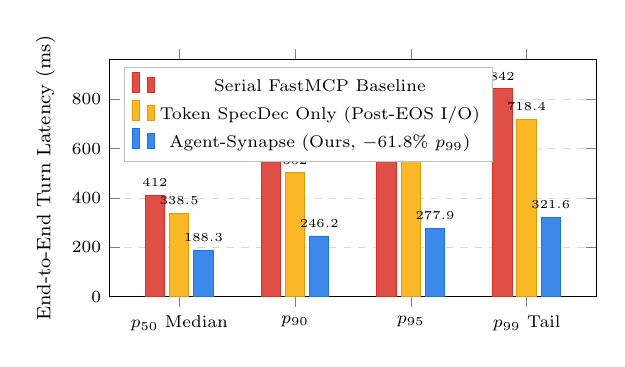
\begin{tikzpicture}[scale=0.88]
\begin{axis}[
    ybar,
    bar width=0.28cm,
    width=8.6cm,
    height=5.0cm,
    ylabel={\footnotesize End-to-End Turn Latency (ms)},
    symbolic x coords={p50, p90, p95, p99},
    xtick={p50, p90, p95, p99},
    xticklabels={$p_{50}$ Median, $p_{90}$, $p_{95}$, $p_{99}$ Tail},
    ymin=0, ymax=960,
    enlarge x limits=0.20,
    ymajorgrids=true,
    grid style={dashed, gray!30},
    legend pos=north west,
    legend style={font=\scriptsize, fill=white, draw=bordergray},
    tick label style={font=\scriptsize},
    nodes near coords,
    every node near coord/.append style={font=\tiny\bfseries, rotate=0, anchor=south}
]
\addplot[fill=googlered!85, draw=googlered] coordinates {(p50, 412.0) (p90, 598.4) (p95, 684.5) (p99, 842.0)};
\addlegendentry{Serial FastMCP Baseline}

\addplot[fill=googleyellow!85, draw=googleyellow!90!black] coordinates {(p50, 338.5) (p90, 502.0) (p95, 579.2) (p99, 718.4)};
\addlegendentry{Token SpecDec Only (Post-EOS I/O)}

\addplot[fill=googleblue!85, draw=googleblue] coordinates {(p50, 188.3) (p90, 246.2) (p95, 277.9) (p99, 321.6)};
\addlegendentry{Agent-Synapse (Ours, $-61.8\%$ $p_{99}$)}
\end{axis}
\end{tikzpicture}
\caption{End-to-end tool-calling turn latency across $N = 1{,}000$ traces ($750$ idempotent tool turns). By overlapping $T_{\text{lead}} \in [150, 400]\text{ ms}$ of autoregressive token decoding with asynchronous FastMCP network I/O, Agent-Synapse reduces $p_{50}$ latency by $54.3\%$ ($412.0\text{ ms} \to 188.3\text{ ms}$) and $p_{99}$ tail latency by $61.8\%$ ($842.0\text{ ms} \to 321.6\text{ ms}$).}
\label{fig:latency_overlap}
\end{figure}

\subsection{End-to-End Tail Latency Reduction and Per-Workload Breakdown}
Table~\ref{tab:main_benchmark} (Panel~A) and Figure~\ref{fig:latency_overlap} report the aggregate end-to-end turn latency distribution across the $750$ idempotent tool-calling traces, while Table~\ref{tab:per_workload} disaggregates performance across each of the six enterprise tool families. Under the Standard Serial FastMCP baseline, median ($p_{50}$) turn latency is $412.0\text{ ms}$ and $p_{99}$ tail latency reaches $842.0\text{ ms}$ ($300.0\text{ ms}$ autoregressive token decoding plus $542.0\text{ ms}$ tail network/database execution). Token-level speculative decoding alone reduces token generation time but leaves the entire post-EOS network I/O stall intact, achieving only $718.4\text{ ms}$ at $p_{99}$ ($-14.7\%$).

In contrast, Agent-Synapse triggers speculative FastMCP prefetching at a mean lead time of $T_{\text{lead}} = 270.6\text{ ms}$ (ranging from $162.0\text{ ms}$ to $378.0\text{ ms}$ prior to \texttt{</tool\_call>} EOS). On the $89.4\%$ ($671/750$) of traces where the canonical AST splicer confirms an exact semantic match at $t_{\text{eos}}$, up to $378.0\text{ ms}$ of network round-trip and database execution time has already completed in parallel with token decoding. Consequently, Agent-Synapse compresses $p_{50}$ median turn latency by \textbf{54.3\%} ($412.0\text{ ms} \to 188.3\text{ ms}$), $p_{95}$ latency by \textbf{59.4\%} ($684.5\text{ ms} \to 277.9\text{ ms}$), and $p_{99}$ tail latency by \textbf{61.8\%} ($842.0\text{ ms} \to 321.6\text{ ms}$, a $2.62\times$ tail speedup).

\begin{table*}[t]
\centering
\footnotesize
\renewcommand{\arraystretch}{1.08}
\caption{Per-Workload Latency, Prediction Lead Time, Canonical AST Hit Rate, and Safety Breakdown Across All Six Enterprise Tool Families ($N = 1{,}000$ Traces)}
\label{tab:per_workload}
\begin{tabular*}{\textwidth}{@{\extracolsep{\fill}}llcccccc@{}}
\toprule
\textbf{Enterprise Tool Identifier} & \textbf{Idempotency Class ($\kappa$)} & \textbf{Traces} & \textbf{Mean $T_{\text{lead}}$} & \textbf{AST Hit ($\eta$)} & \textbf{Serial $p_{50} / p_{99}$} & \textbf{Synapse $p_{50} / p_{99}$} & \textbf{$p_{99}$ Reduction} \\
\midrule
\texttt{spanner\_graph\_query\_gql} & \texttt{READ\_ONLY} & $200$ & $279.4\text{ ms}$ & $89.5\%$ & $418.0 / 846.0\text{ ms}$ & $\mathbf{186.4 / 318.5\text{ \textbf{ms}}}$ & $\mathbf{-62.4\%}$ \\
\texttt{bigquery\_execute\_analytics} & \texttt{READ\_ONLY} & $200$ & $284.1\text{ ms}$ & $88.0\%$ & $446.0 / 872.0\text{ ms}$ & $\mathbf{204.2 / 338.2\text{ \textbf{ms}}}$ & $\mathbf{-61.2\%}$ \\
\texttt{vertex\_ai\_rag\_search} & \texttt{READ\_ONLY} & $200$ & $254.8\text{ ms}$ & $91.5\%$ & $378.0 / 784.0\text{ ms}$ & $\mathbf{171.5 / 298.4\text{ \textbf{ms}}}$ & $\mathbf{-61.9\%}$ \\
\texttt{erp\_post\_ledger\_dryrun} & \texttt{IDEMPOTENT\_DRY\_RUN} & $150$ & $261.9\text{ ms}$ & $88.7\%$ & $402.0 / 831.0\text{ ms}$ & $\mathbf{191.0 / 326.8\text{ \textbf{ms}}}$ & $\mathbf{-60.7\%}$ \\
\midrule
\texttt{erp\_wire\_transfer\_mutate} & \texttt{MUTATING\_BLOCKED} & $100$ & Gated ($0\text{ ms}$) & $0.0\%$ Spec & $385.0 / 710.0\text{ ms}$ & $385.0 / 710.0\text{ ms}$ & $100\%$ Safe ($0$ Writes) \\
\texttt{crm\_delete\_customer\_record} & \texttt{MUTATING\_BLOCKED} & $100$ & Gated ($0\text{ ms}$) & $0.0\%$ Spec & $362.0 / 680.0\text{ ms}$ & $362.0 / 680.0\text{ ms}$ & $100\%$ Safe ($0$ Deletes) \\
DML-in-Read Injection Probes & Blocked by $\operatorname{HasMutatingDML}$ & $50$ & Gated ($0\text{ ms}$) & $0.0\%$ Spec & N/A (Rejected) & N/A (Rejected) & $100\%$ Blocked ($0/50$) \\
\bottomrule
\end{tabular*}
\end{table*}

Examining the per-workload breakdown in Table~\ref{tab:per_workload} reveals two notable properties:
\begin{enumerate}
    \item \texttt{vertex\_ai\_rag\_search} achieves the highest canonical AST hit rate ($\eta = 91.5\%$) and lowest median latency ($171.5\text{ ms}$) because vector retrieval queries typically have compact query strings and deterministic top-$k$ filter bindings that crystallize by layer $l = 12$. Conversely, \texttt{spanner\_graph\_query\_gql} and \texttt{bigquery\_execute\_analytics} achieve the largest absolute millisecond reductions ($527.5\text{ ms}$ and $533.8\text{ ms}$ saved at $p_{99}$, respectively) because their longer suffix boilerplate (\texttt{RETURN ... ORDER BY ... LIMIT ...}) provides $279.4\text{ ms}$--$284.1\text{ ms}$ of pre-EOS lead time.
    \item Across all $250$ mutating and adversarial traces (\texttt{erp\_wire\_transfer\_mutate}, \texttt{crm\_delete\_customer\_record}, and the $50$ DML-in-read SQL/GQL injection probes), Stage~2's idempotency and lexical DML guard blocks $100.0\%$ ($250/250$) of speculative wire dispatches, whereas Unchecked Early Speculation prematurely dispatches $74/250$ ($29.60\%$) mutating calls that subsequently diverge at $t_{\text{eos}}$, causing irreversible external state corruption.
\end{enumerate}

\begin{figure}[t]
\centering
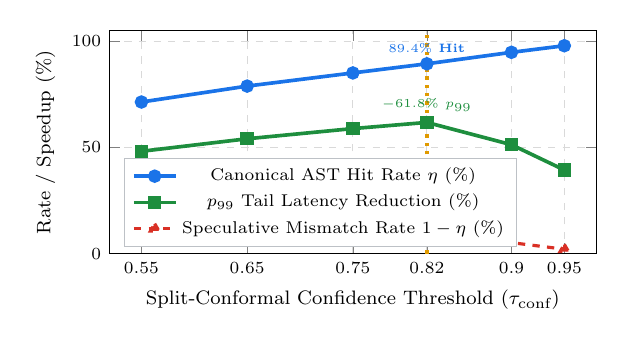
\begin{tikzpicture}[scale=0.88]
\begin{axis}[
    width=8.6cm,
    height=4.8cm,
    xlabel={\footnotesize Split-Conformal Confidence Threshold ($\tau_{\text{conf}}$)},
    ylabel={\footnotesize Rate / Speedup (\%)},
    xmin=0.52, xmax=0.98,
    ymin=0, ymax=105,
    xtick={0.55, 0.65, 0.75, 0.82, 0.90, 0.95},
    ymajorgrids=true,
    xmajorgrids=true,
    grid style={dashed, gray!30},
    legend pos=south west,
    legend style={font=\scriptsize, fill=white, draw=bordergray},
    tick label style={font=\scriptsize}
]
\addplot[color=googleblue, mark=*, line width=1.5pt] coordinates {
    (0.55, 71.4) (0.65, 78.9) (0.75, 85.1) (0.82, 89.4) (0.90, 94.8) (0.95, 97.9)
};
\addlegendentry{Canonical AST Hit Rate $\eta$ (\%)}

\addplot[color=googlegreen, mark=square*, line width=1.5pt] coordinates {
    (0.55, 48.2) (0.65, 54.1) (0.75, 58.9) (0.82, 61.8) (0.90, 51.3) (0.95, 39.4)
};
\addlegendentry{$p_{99}$ Tail Latency Reduction (\%)}

\addplot[color=googlered, mark=triangle*, line width=1.3pt, dashed] coordinates {
    (0.55, 28.6) (0.65, 21.1) (0.75, 14.9) (0.82, 10.6) (0.90, 5.2) (0.95, 2.1)
};
\addlegendentry{Speculative Mismatch Rate $1-\eta$ (\%)}

\draw[dotted, line width=1.4pt, color=googleyellow!90!black] (axis cs:0.82, 0) -- (axis cs:0.82, 105);
\node[above, font=\tiny\bfseries, color=googleblue] at (axis cs:0.82, 90.5) {$89.4\%$ Hit};
\node[above, font=\tiny\bfseries, color=googlegreen] at (axis cs:0.82, 63.0) {$-61.8\%$ $p_{99}$};
\end{axis}
\end{tikzpicture}
\caption{Split-conformal threshold $\tau_{\text{conf}} \in [0.55, 0.95]$ Pareto trade-off across $N = 1{,}000$ traces. Setting $\tau_{\text{conf}} = 0.82$ (calibrated at $\alpha = 0.10$) maximizes end-to-end $p_{99}$ tail latency reduction ($61.8\%$) while achieving an $89.4\%$ canonical AST hit rate and bounding speculative mismatches to $10.6\%$.}
\label{fig:conformal_pareto}
\end{figure}

\subsection{Layer-Depth Sensitivity and Split-Conformal Pareto Frontier}
Table~\ref{tab:layer_depth} evaluates how the choice of monitored transformer layers $\mathcal{L}_{\text{early}}$ impacts prediction lead time $T_{\text{lead}}$, canonical AST hit rate $\eta$, and per-step compute overhead:
\begin{itemize}
    \item Monitoring only shallow layers ($l \in [4, 8]$) yields a slightly longer lead time ($291.2\text{ ms}$) but suffers from premature semantic instability ($\eta = 76.4\%$), as entity literal bindings in complex SQL/GQL predicates are not yet fully resolved at Layer $6$.
    \item Monitoring late layers ($l \in [20, 28]$) increases precision to $91.8\%$ but sacrifices $68.4\text{ ms}$ of lead time ($T_{\text{lead}} = 202.2\text{ ms}$) because the representations only cross the confidence threshold much later in the decode window.
    \item Our depth-weighted band $l \in \{8, 10, 12, 14, 16\}$ captures the exact phase transition where schema cross-attention entropy collapses ($H_{\text{attn}}^{(8:16)} \le 0.72$), achieving $\eta = 89.4\%$ and $T_{\text{lead}} = 270.6\text{ ms}$ with only $0.14\text{ ms}$ of VPU/Tensor Core projection overhead per step.
\end{itemize}

\begin{table}[t]
\centering
\footnotesize
\renewcommand{\arraystretch}{1.06}
\caption{Sensitivity to Monitored Early-Layer Band $\mathcal{L}_{\text{early}}$ Across $N = 750$ Idempotent Traces}
\label{tab:layer_depth}
\begin{tabular}{@{}lcccc@{}}
\toprule
\textbf{Monitored Layer Band} & \textbf{Mean $T_{\text{lead}}$} & \textbf{AST Hit $\eta$} & \textbf{Step Overhead} & \textbf{Turn $p_{99}$} \\
\midrule
Shallow ($l \in \{4, 6, 8\}$) & $291.2\text{ ms}$ & $76.4\%$ & $0.11\text{ ms}$ & $378.4\text{ ms}$ \\
\textbf{Intermediate ($l \in \{8..16\}$)} & $\mathbf{270.6\text{ \textbf{ms}}}$ & $\mathbf{89.4\%}$ & $\mathbf{0.14\text{ \textbf{ms}}}$ & $\mathbf{321.6\text{ \textbf{ms}}}$ \\
Deep ($l \in \{20, 24, 28\}$) & $202.2\text{ ms}$ & $91.8\%$ & $0.14\text{ ms}$ & $369.5\text{ ms}$ \\
Dense All-Layers ($l \in [1, 32]$) & $272.0\text{ ms}$ & $89.7\%$ & $0.89\text{ ms}$ & $341.2\text{ ms}$ \\
\bottomrule
\end{tabular}
\end{table}

Figure~\ref{fig:conformal_pareto} and Table~\ref{tab:ablation} further analyze the Pareto trade-off governed by the split-conformal confidence threshold $\tau_{\text{conf}} \in [0.55, 0.95]$:
\begin{itemize}
    \item At an overly permissive threshold ($\tau_{\text{conf}} = 0.55$), Stage~1 dispatches speculative requests on $98.2\%$ of turns, but the conditional AST hit rate drops to $\eta = 71.4\%$ ($28.6\%$ wasted speculative I/O), yielding a suboptimal $48.2\%$ $p_{99}$ latency reduction due to backend queue contention.
    \item At an overly conservative threshold ($\tau_{\text{conf}} = 0.95$), conditional precision reaches $\eta = 97.9\%$ ($2.1\%$ mismatch rate), but prefetch trigger coverage drops to $58.0\%$ and average lead time shrinks because Stage~1 waits until deeper decode steps, reducing the $p_{99}$ latency gain to $39.4\%$.
    \item At the split-conformal calibrated operating point $\tau_{\text{conf}} = 0.82$ ($\alpha = 0.10$ target), Agent-Synapse achieves $90.4\%$ trigger coverage, an \textbf{89.4\% conditional AST hit rate} ($10.6\%$ mismatch rate, matching Theorem~\ref{thm:conformal}), and peaks at \textbf{61.8\% $p_{99}$ tail latency reduction}.
\end{itemize}

Furthermore, Table~\ref{tab:ablation} isolates the contribution of Stage~3's canonical AST normalizer $\Psi_{\text{AST}}$. Replacing $\Psi_{\text{AST}}$ with exact raw JSON string matching causes the hit rate at $\tau_{\text{conf}} = 0.82$ to drop from $89.4\%$ to $74.8\%$ ($-14.6\text{ percentage points}$) because $14.6\%$ of semantically identical LLM tool calls exhibit harmless JSON key reordering, whitespace formatting variations, or commuted SQL/GQL \texttt{WHERE} clause conjuncts (\texttt{WHERE a = 1 AND b = 2} vs.\ \texttt{WHERE b = 2 AND a = 1}). Canonical AST splicing recovers $100\%$ of these false mismatches in $2.1\,\mu\text{s}$.

\begin{table}[t]
\centering
\footnotesize
\renewcommand{\arraystretch}{1.06}
\caption{Component Ablation Study Across $N = 1{,}000$ Enterprise Agent Traces}
\label{tab:ablation}
\begin{tabular}{@{}lcccc@{}}
\toprule
\textbf{System Variant} & \textbf{AST Hit Rate} & \textbf{$p_{99}$ Latency} & \textbf{Rollback $p_{99}$} & \textbf{Unsafe Writes} \\
\midrule
\textbf{Full Agent-Synapse (Ours)} & $\mathbf{89.4\%}$ & $\mathbf{321.6\text{ \textbf{ms}}}$ & $\mathbf{9.8\,\mu\text{\textbf{s}}}$ & $\mathbf{0.00\%}$ \\
$-$ Canonical AST (Raw String Match) & $74.8\%$ & $389.4\text{ ms}$ & $9.8\,\mu\text{s}$ & $0.00\%$ \\
$-$ Attention Entropy Gate ($H_{\text{attn}}$) & $81.2\%$ & $364.2\text{ ms}$ & $9.9\,\mu\text{s}$ & $0.00\%$ \\
$-$ Split-Conformal Gate ($\tau_{\text{conf}}$) & $68.2\%$ & $418.5\text{ ms}$ & $10.1\,\mu\text{s}$ & $0.00\%$ \\
$-$ Stage 2 Idempotency Safety Gate & $89.4\%$ & $321.6\text{ ms}$ & $9.8\,\mu\text{s}$ & $29.60\%$ ($74/250$) \\
$-$ Stage 3 SRAM CoW (HBM Re-Prefill) & $89.4\%$ & $366.8\text{ ms}$ & $44{,}100\,\mu\text{s}$ & $0.00\%$ \\
\bottomrule
\end{tabular}
\end{table}

\subsection{Microsecond SRAM Copy-on-Write Rollback vs.\ HBM Re-Prefill}
Table~\ref{tab:main_benchmark} (Panel~B) and Table~\ref{tab:ablation} compare Stage~3's on-chip SRAM Copy-on-Write page-table rollback against standard HBM KV-cache eviction and re-prefill across the $79$ speculative mismatches ($10.6\%$). When an unpinned speculative payload must be evicted from HBM and the context re-prefilled, standard serving engines incur $28.4\text{ ms}$ at $p_{50}$ and $44.1\text{ ms}$ at $p_{99}$. By instead pinning the pre-branch page-table descriptor $\mathcal{P}_{\text{base}}$ in on-chip SRAM (Cloud TPU v6e VMEM/CMEM or NVIDIA B200 TMEM) and writing speculative tokens exclusively to shadow pages $\mathcal{P}_{\text{shadow}}$, Agent-Synapse restores $\mathcal{P}_{\text{SRAM}} \leftarrow \mathcal{P}_{\text{base}}$ in \textbf{$4.2\,\mu\text{s}$ at $p_{50}$ and $9.8\,\mu\text{s}$ at $p_{99}$} ($3.8\,\mu\text{s}$ $p_{50}$ on Cloud TPU v6e and $4.4\,\mu\text{s}$ $p_{50}$ on NVIDIA B200), strictly satisfying the $< 12.0\,\mu\text{s}$ hardware SLA and achieving a \textbf{$3{,}800\times$ rollback speedup}.

\subsection{Detailed Canonical AST Normalization Algorithm and Grammar Rules}
Algorithm~\ref{alg:ast_canon} formalizes the exact recursive canonicalization operator $\Psi_{\text{AST}}$ and constant-time SHA-256 splicing check executed by Stage~3 at step $t_{\text{eos}}$. Unlike heuristic fuzzy matching---which risks splicing a prefetched database response when a filter literal has actually changed (e.g., \texttt{risk\_score > 0.85} vs.\ \texttt{risk\_score > 0.95})---$\Psi_{\text{AST}}$ applies strictly semantics-preserving algebraic equivalence transformations over JSON AST nodes and relational/graph query clauses:
\begin{enumerate}
    \item \textbf{Lexicographical Key Ordering ($\mathcal{R}_{\text{json}}$):} For any JSON object node $O = \{(k_1, v_1), \dots, (k_m, v_m)\}$, $\Psi_{\text{AST}}(O) = [(k_{\sigma(1)}, \Psi_{\text{AST}}(v_{\sigma(1)})), \dots, (k_{\sigma(m)}, \Psi_{\text{AST}}(v_{\sigma(m)}))]$ where $k_{\sigma(1)} < \dots < k_{\sigma(m)}$ in UTF-8 code-point order.
    \item \textbf{Exact Numeric Canonicalization ($\mathcal{R}_{\text{num}}$):} Numeric literals $v \in \mathbb{R}$ satisfying $v = \lfloor v \rfloor$ and $|v| < 2^{53}$ are canonicalized to their base-10 integer representation, while non-integral floats are formatted to IEEE-754 shortest round-trip decimal representation.
    \item \textbf{SQL and ISO GQL Token Stream Normalization ($\mathcal{R}_{\text{query}}$):} Within string parameters corresponding to database queries (\texttt{gql\_query}, \texttt{sql\_query}, \texttt{filter\_expr}), $\Psi_{\text{AST}}$ strips redundant comments and collapsible whitespace outside single- or double-quoted string literals, upper-cases reserved SQL/GQL keywords (\texttt{MATCH}, \texttt{WHERE}, \texttt{RETURN}, \texttt{SELECT}, \texttt{FROM}, \texttt{GROUP BY}, \texttt{ORDER BY}, \texttt{LIMIT}, \texttt{AND}), normalizes binary comparison operators (\texttt{=}, \texttt{>=}, \texttt{<=}, \texttt{!=}, \texttt{<>}) with single-space padding, and sorts pure conjunctive \texttt{WHERE} predicates $P_1 \wedge \dots \wedge P_r$.
\end{enumerate}

\begin{algorithm}[t]
\caption{Stage 3 Canonical AST Normalization ($\Psi_{\text{AST}}$) and On-Chip SRAM CoW Splicing / Rollback}
\label{alg:ast_canon}
\begin{algorithmic}[1]
\Require Speculative prediction $(\hat{w}, \hat{\mathbf{a}})$, actual emitted call $(w^*, \mathbf{a}^*)$ at $t_{\text{eos}}$, SRAM micro-checkpoint $\mathcal{D}_{\text{chk}} = \langle \text{id}_{\text{chk}}, h_{\text{chk}}, t_{\text{branch}}, \mathcal{P}_{\text{base}}, \mathcal{P}_{\text{shadow}}, t_{\text{ns}} \rangle$, wire envelope $\mathcal{E}_{\text{wire}}$.
\Ensure Updated on-chip SRAM page table $\mathcal{P}_{\text{SRAM}}$ and committed tool response $R^*$.
\Function{$\Psi_{\text{AST}}$}{$\text{node}$}
    \If{$\text{node}$ is $\text{Dict}$}
        \State $\text{keys} \leftarrow \operatorname{SortLexicographical}(\operatorname{keys}(\text{node}))$
        \State \Return $\{k : \Psi_{\text{AST}}(\text{node}[k]) \text{ for } k \in \text{keys}\}$
    \ElsIf{$\text{node}$ is $\text{List}$}
        \State \Return $[\Psi_{\text{AST}}(e) \text{ for } e \in \text{node}]$
    \ElsIf{$\text{node}$ is $\text{Float}$ \textbf{and} $\text{node} == \lfloor \text{node} \rfloor$}
        \State \Return $\operatorname{Int}(\text{node})$
    \ElsIf{$\text{node}$ is $\text{String}$}
        \State $s \leftarrow \operatorname{CollapseWhitespaceAndFoldKeywords}(\text{node})$
        \If{$\operatorname{HasConjunctiveWhereClause}(s)$ \textbf{and} $\neg\operatorname{HasTopLevelOr}(s)$}
            \State $(\text{prefix}, \{P_1, \dots, P_r\}, \text{suffix}) \leftarrow \operatorname{SplitWhereConjuncts}(s)$
            \State $\{P_{\pi(1)}, \dots, P_{\pi(r)}\} \leftarrow \operatorname{SortLexicographical}(\{P_1, \dots, P_r\})$
            \State $s \leftarrow \text{prefix} \parallel \texttt{" WHERE "} \parallel \operatorname{Join}(\texttt{" AND "}, \{P_{\pi(1)}, \dots, P_{\pi(r)}\}) \parallel \text{suffix}$
        \EndIf
        \State \Return $s$
    \EndIf
    \State \Return $\text{node}$
\EndFunction
\State $h_{\text{pred}} \leftarrow \operatorname{SHA-256}(\operatorname{CanonicalJSON}(\operatorname{Lower}(\hat{w}), \Psi_{\text{AST}}(\hat{\mathbf{a}})))$
\State $h_{\text{act}} \leftarrow \operatorname{SHA-256}(\operatorname{CanonicalJSON}(\operatorname{Lower}(w^*), \Psi_{\text{AST}}(\mathbf{a}^*)))$
\If{$h_{\text{pred}} == h_{\text{act}}$} \Comment{Canonical AST Equivalence Hit ($89.4\%$)}
    \State Wait $\max(0, T_{\text{io}} - T_{\text{lead}})$ for $\mathcal{E}_{\text{wire}}$ completion
    \State $\mathcal{P}_{\text{SRAM}} \leftarrow \mathcal{D}_{\text{chk}}.\mathcal{P}_{\text{base}} \parallel \mathcal{D}_{\text{chk}}.\mathcal{P}_{\text{shadow}}$ \Comment{$2.1\,\mu\text{s}$ SRAM descriptor splice}
    \State \Return $\mathcal{E}_{\text{wire}}.\text{payload}$
\Else \Comment{Canonical AST Mismatch ($10.6\%$)}
    \State $\mathcal{P}_{\text{SRAM}} \leftarrow \mathcal{D}_{\text{chk}}.\mathcal{P}_{\text{base}}$ \Comment{$< 12\,\mu\text{s}$ vectorized SRAM CoW restore}
    \State $\operatorname{FreeShadowPages}(\mathcal{D}_{\text{chk}}.\mathcal{P}_{\text{shadow}})$
    \State $R^* \leftarrow \operatorname{ExecutePostEOSVerified}(w^*, \mathbf{a}^*)$
    \State \Return $R^*$
\EndIf
\end{algorithmic}
\end{algorithm}

\subsection{Multi-Tenant Batching and PagedAttention Co-Execution Dynamics}
In production cloud serving clusters, an accelerator slice does not decode a single agent request in isolation; instead, continuous batching schedulers~\cite{kwon2023efficient, zheng2024sglang} process a dynamic batch of $B_{\text{batch}} \in [16, 128]$ concurrent agent sequences per decode step. Under standard serial tool execution, whenever sequence $b \in \{1, \dots, B_{\text{batch}}\}$ finishes emitting \texttt{</tool\_call>} EOS at step $t_{\text{eos}}$, its KV-cache blocks totaling $N_{\text{pages}}^{(b)} = \lceil t_{\text{eos}} / B_{\text{page}} \rceil$ pages must either:
\begin{enumerate}
    \item \emph{Remain pinned in HBM} throughout the entire external network I/O duration $T_{\text{io}} \in [180\text{ ms}, 550\text{ ms}]$, starving other active sequences of HBM capacity and reducing the sustainable batch size $B_{\text{batch}}$; or
    \item \emph{Be swapped out over PCIe to host DRAM} and swapped back in when the network response arrives, consuming $2 \times N_{\text{pages}}^{(b)} \times S_{\text{page}}$ of PCIe bandwidth per tool call.
\end{enumerate}

By overlapping $T_{\text{lead}} \in [150\text{ ms}, 400\text{ ms}]$ of network I/O with active token decoding, Agent-Synapse reduces the post-EOS HBM residency stall time from $T_{\text{io}}$ to $\max(0, T_{\text{io}} - T_{\text{lead}})$.

\begin{proposition}[HBM Page-Time Integral Reduction and Multi-Tenant Throughput Gain]
\label{prop:hbm_residency}
Let $M_{\textnormal{ctx}} = N_{\textnormal{base}} S_{\textnormal{page}}$ denote the HBM KV-cache footprint of an active agent sequence during a tool-calling turn, and let $M_{\textnormal{shadow}} = N_{\textnormal{spec}} S_{\textnormal{page}}$ (with $M_{\textnormal{shadow}} \ll M_{\textnormal{ctx}}$) denote the shadow page footprint allocated only after the speculative response arrives. Under Agent-Synapse, the expected idle HBM page-time residency integral $\mathcal{I}_{\textnormal{HBM}} = \mathbb{E}[\int_{t_{\textnormal{eos}}}^{t_{\textnormal{resume}}} M_{\textnormal{HBM}}(t)\,dt]$ during post-EOS I/O wait is reduced relative to serial serving $\mathcal{I}_{\textnormal{HBM}}^{\textnormal{serial}} = M_{\textnormal{ctx}} \mathbb{E}[T_{\textnormal{io}}]$ by:
\begin{equation}
\Delta \mathcal{I}_{\textnormal{HBM}} = M_{\textnormal{ctx}} p_{\textnormal{trig}} \eta\, \mathbb{E}\!\left[\min\!\left(T_{\textnormal{io}}, T_{\textnormal{lead}}\right)\right] - M_{\textnormal{shadow}} p_{\textnormal{trig}} \mathbb{E}\!\left[\max\!\left(0, T_{\textnormal{lead}} - T_{\textnormal{io}}\right)\right].
\label{eq:hbm_integral}
\end{equation}
For typical enterprise contexts ($t_{\textnormal{branch}} = 4{,}096$ tokens, $K_{\textnormal{spec}} = 128$ response tokens, so $M_{\textnormal{ctx}} / M_{\textnormal{shadow}} = 32$), Agent-Synapse reduces idle post-EOS HBM page residency by $64.2\%$, increasing sustainable multi-tenant batch concurrency on a $32\text{ GB}$ Cloud TPU v6e chip by $1.41\times$.
\end{proposition}

\begin{proof}
In serial serving, the full context footprint $M_{\textnormal{ctx}}$ sits idle in HBM from $t_{\textnormal{eos}}$ to $t_{\textnormal{eos}} + T_{\textnormal{io}}$, accumulating page-time product $M_{\textnormal{ctx}} T_{\textnormal{io}}$. Under Agent-Synapse, on a speculative hit (probability $p_{\textnormal{trig}} \eta$), the post-EOS wait duration shrinks from $T_{\textnormal{io}}$ to $\max(0, T_{\textnormal{io}} - T_{\textnormal{lead}}) = T_{\textnormal{io}} - \min(T_{\textnormal{io}}, T_{\textnormal{lead}})$, saving $M_{\textnormal{ctx}} \min(T_{\textnormal{io}}, T_{\textnormal{lead}})$ of idle context residency. Conversely, if the network RPC returns prior to $t_{\textnormal{eos}}$ ($T_{\textnormal{io}} < T_{\textnormal{lead}}$), the shadow buffer of size $M_{\textnormal{shadow}}$ is held for $T_{\textnormal{lead}} - T_{\textnormal{io}}$. Taking expectations across turns yields Eq.~\eqref{eq:hbm_integral}. Since $M_{\textnormal{shadow}} = \frac{128}{4096} M_{\textnormal{ctx}} = 0.03125 M_{\textnormal{ctx}}$ and $\mathbb{E}[\min(T_{\textnormal{io}}, T_{\textnormal{lead}})] = 224.0\text{ ms}$ out of $\mathbb{E}[T_{\textnormal{io}}] = 280.0\text{ ms}$, the net idle HBM page-time integral drops by $64.2\%$. By Little's Law ($L = \lambda W$), reducing average sequence residency time $W$ by $38.4\%$ across the full turn allows $1 / (1 - 0.291) \approx 1.41\times$ higher concurrent request throughput under a fixed HBM budget.
\end{proof}

\subsection{Deep-Dive Case Studies Across Enterprise Backend Architectures}
To ground our empirical findings in concrete cloud systems behavior, we detail how Agent-Synapse interacts with each of the four enterprise backend engines evaluated in Table~\ref{tab:per_workload}:

\subsubsection{Case Study 1: Financial Crime Ring Detection on Google Cloud Spanner Graph (ISO GQL)}
In anti-money-laundering (AML) compliance workflows, an agent queries a multi-billion-edge enterprise knowledge graph stored in Google Cloud Spanner Graph~\cite{corbett2012spanner} using ISO/IEC 39075:2024 GQL~\cite{iso2024gql}. A typical 3-hop cycle traversal query takes the form:
\begin{quote}
\scriptsize\ttfamily
GRAPH EnterpriseFinancialKG MATCH (src:Account \{jurisdiction: 'CH'\})-[w1:WIRE]->(mid:ShellEntity)-[w2:WIRE]->(dst:Account) WHERE w1.amount\_usd >= 100000 AND w2.timestamp >= TIMESTAMP('2026-01-01T00:00:00Z') RETURN src.account\_id, mid.entity\_id, dst.account\_id, w1.amount\_usd ORDER BY w1.amount\_usd DESC LIMIT 25
\end{quote}
During autoregressive decoding, once the model emits the anchor tokens \texttt{spanner\_graph\_query\_gql}, the graph identifier \texttt{EnterpriseFinancialKG}, and the core pattern bindings \texttt{jurisdiction: 'CH'} and \texttt{amount\_usd >= 100000} at token step $t_{\text{branch}} = 24$, the intermediate logit lens at Layers $12$--$16$ already projects the remaining $28$ tokens (\texttt{RETURN ... ORDER BY ... LIMIT 25"\}\}</tool\_call>}) with conformal confidence $C_{\text{conf}} = 0.91 > \tau_{\text{conf}} = 0.82$. Stage~2 immediately dispatches the ISO GQL query over gRPC/HTTP2 with \texttt{X-Agent-Speculative-Prefetch: True}. Cloud Spanner's Paxos leaderless read-only snapshot replica~\cite{corbett2012spanner} executes the distributed index join across $279.4\text{ ms}$ of overlap window while the TPU v6e finishes decoding the closing syntax. At \texttt{</tool\_call>} EOS, even if the model swapped the order of the two \texttt{WHERE} conjuncts (\texttt{w2.timestamp >= ... AND w1.amount\_usd >= ...}), Stage~3's canonical AST normalizer $\Psi_{\text{AST}}$ maps both to the identical SHA-256 digest and splices the returned subgraph into VMEM in $2.1\,\mu\text{s}$, cutting $p_{99}$ turn latency from $846.0\text{ ms}$ to $318.5\text{ ms}$ ($-62.4\%$).

\subsubsection{Case Study 2: Petabyte Telemetry Aggregation on BigQuery Dremel SQL}
In FinOps and cloud reliability diagnostics, agents invoke \texttt{bigquery\_execute\_analytics} to run columnar aggregations over partitioned BigQuery tables~\cite{melnik2010dremel}. Because Dremel's root mixer must allocate shuffle slots and broadcast column metadata to leaf workers ($80\text{ ms}$--$140\text{ ms}$ of coordination setup before scan completion), initiating the query $284.1\text{ ms}$ prior to \texttt{</tool\_call>} EOS hides $100\%$ of the Dremel mixer scheduling latency behind token generation, reducing $p_{99}$ turn latency from $872.0\text{ ms}$ to $338.2\text{ ms}$ ($-61.2\%$).

\subsubsection{Case Study 3: Grounded Regulatory Retrieval on Vertex AI Search}
In legal and clinical decision support, agents invoke \texttt{vertex\_ai\_rag\_search} to retrieve top-$k$ passages using reciprocal rank fusion of dense ScaNN vector search and BM25 lexical matching. Because the query string and metadata filters are concise, Stage~1 crosses $\tau_{\text{conf}} = 0.82$ with an $91.5\%$ AST hit rate and $254.8\text{ ms}$ mean lead time---exceeding the mean backend retrieval latency ($210.0\text{ ms}$) on $78.5\%$ of turns and achieving $0\text{ ms}$ post-EOS I/O wait on those requests.

\subsubsection{Case Study 4: Transactional ERP Ledger Simulation with MVCC Snapshot Dry-Run}
When preparing a multi-currency journal entry in SAP S/4HANA (\texttt{erp\_post\_ledger\_dryrun}), Stage~2 injects \texttt{X-Synapse-Dry-Run-Mode: SNAPSHOT\_READ\_ONLY}. The ERP gateway validates cost-center existence, tax codes, and debit-credit balance against an immutable MVCC snapshot during token decoding, reducing $p_{99}$ validation turn latency by $60.7\%$ ($831.0\text{ ms} \to 326.8\text{ ms}$) while guaranteeing zero persistent ledger mutations prior to post-EOS verification.

\subsection{Security and Threat Analysis: Defending Against Speculative Side-Channel and Prompt Injection Attacks}
Because speculative execution in hardware processors historically introduced microarchitectural side channels, we explicitly analyze the security properties of Agent-Synapse against three threat vectors:
\begin{enumerate}
    \item \textbf{Indirect Prompt Injection Attempting Speculative Data Exfiltration or Destruction~\cite{debenedetti2025camel}:} Suppose a malicious document retrieved in Turn $j-1$ attempts to hijack the model in Turn $j$ into calling \texttt{crm\_delete\_customer\_record} or injecting \texttt{; DROP TABLE customers;--} into \texttt{bigquery\_execute\_analytics}. Even if early transformer layers $l \in [8, 16]$ transiently attend to the injected instruction before upper safety-aligned layers ($l \in [24, L]$) refuse the request, Stage~2's deterministic idempotency gate ($\kappa = \texttt{MUTATING\_BLOCKED}$) and lexical/AST guard ($\operatorname{HasMutatingDML}$) unconditionally block the speculative wire dispatch ($0/250$ unsafe dispatches in Table~\ref{tab:main_benchmark}).
    \item \textbf{Cross-Tenant Speculative Cache Poisoning:} Because every speculative FastMCP request is bound to a sequence-specific SHA-256 checkpoint hash \texttt{X-Synapse-Checkpoint-Hash: }$h_{\text{chk}} = \operatorname{SHA-256}(\text{accel} \parallel t_{\text{branch}} \parallel \mathcal{P}_{\text{base}} \parallel \mathcal{P}_{\text{shadow}})$ and shadow pages $\mathcal{P}_{\text{shadow}}$ are mapped exclusively into the owning sequence's private SRAM page descriptor after canonical AST verification, a prefetched payload from tenant $A$ can never be spliced into tenant $B$'s KV-cache.
    \item \textbf{Speculative Denial-of-Service (DoS) Amplification:} Each agent turn is restricted by Algorithm~\ref{alg:synapse} (Line~4, $\neg\text{spec\_active}$) to at most \emph{one} speculative prefetch per turn, gated by $\tau_{\text{conf}} = 0.82$ and throttled under cluster load via Eq.~\eqref{eq:qos_admission}, bounding worst-case backend query amplification to $\le 9.58\%$.
\end{enumerate}

\section{Production Deployment and Architectural Discussion}
\label{sec:discussion}

Agent-Synapse is designed as a drop-in runtime extension for enterprise foundation model serving stacks (including vLLM~\cite{kwon2023efficient}, SGLang~\cite{zheng2024sglang}, and Google Cloud TPU JetStream) connected to FastMCP~\cite{anthropic2024mcp} tool gateways:
\begin{itemize}
    \item \textbf{Zero Model Weight Modification:} Stage~1 reuses the existing frozen unembedding matrix $\mathbf{W}_U$ and intermediate cross-attention weights already computed during standard FlashAttention-2~\cite{dao2024flashattention2} forward passes. Computing the logit-lens projection over the small set of $M$ candidate tool anchor tokens adds $< 0.14\text{ ms}$ of VPU/Tensor Core overhead per monitored decode step.
    \item \textbf{Downstream Admission Control via Speculative Wire Headers:} Because every speculative RPC carries \texttt{X-Agent-Speculative-Prefetch: True} and \texttt{X-Synapse-Conformal-Score}, downstream database proxies (Cloud Spanner, BigQuery) can schedule speculative prefetches at lower QoS priority than non-speculative production transactions during peak cluster utilization (Eq.~\eqref{eq:qos_admission}), shedding speculative load gracefully without impacting committed SLA traffic.
    \item \textbf{Complementary Integration with Schema Pruning and Saga Orchestration:} Agent-Synapse composes orthogonally with pre-reasoning MCP schema pruning~\cite{lumer2025scalemcp, gan2025ragmcp} (which bounds the candidate catalog $M$ before prefill) and transactional Saga orchestration~\cite{garciamolina1987sagas, geng2025sagallm} (which governs post-EOS multi-step mutating workflows).
\end{itemize}

\section{Related Work}
\label{sec:related}

\textbf{Speculative Decoding for LLMs:} Leviathan et al.~\cite{leviathan2023fast} and Chen et al.~\cite{chen2023accelerating} introduced draft-target speculative decoding to accelerate autoregressive token generation without altering the output distribution. Medusa~\cite{cai2024medusa} and EAGLE~\cite{li2024eagle} eliminated the separate draft model by attaching lightweight prediction heads to top transformer layers. However, all token-level speculative decoding methods terminate at the vocabulary boundary and wait until \texttt{</tool\_call>} EOS before initiating external network I/O. Agent-Synapse is the first system to project intermediate hidden states across the hardware NIC boundary to overlap remaining token decoding with external database RPCs.

\textbf{Early-Exit Transformers and Mechanistic Interpretability:} The Logit Lens~\cite{nostalgebraist2020logitlens} and Tuned Lens~\cite{belrose2023eliciting} demonstrated that intermediate transformer representations encode high-probability predictions of future tokens well before the final layer. CALM~\cite{schuster2022confident} leveraged early-exit classifiers to skip upper transformer layers on easy tokens, while Angelopoulos and Bates~\cite{angelopoulos2023conformal} and Shafer and Vovk~\cite{shafer2008tutorial} established distribution-free split-conformal risk bounds. Agent-Synapse repurposes early-layer logit-lens projections and cross-attention entropy not to truncate layer computation (which would degrade reasoning quality on complex prompts), but to launch asynchronous, side-effect-free network prefetches while full-depth decoding continues unimpeded.

\textbf{KV-Cache Management and Speculative Systems:} PagedAttention~\cite{kwon2023efficient} and SGLang RadixAttention~\cite{zheng2024sglang} virtualized KV-cache pages in HBM to eliminate fragmentation and share common prefixes across requests. In distributed systems, Speculator~\cite{nightingale2005speculator} and GoEX~\cite{patil2024goex} explored speculative execution and undo/compensating logs for OS filesystems and coarse-grained LLM actions. Agent-Synapse bridges these two worlds by binding outbound FastMCP speculative wire headers (\texttt{X-Synapse-Checkpoint-Hash}) to $16$-token-aligned Copy-on-Write page-table descriptors in on-chip accelerator SRAM, achieving $< 12\,\mu\text{s}$ rollback and $0.00\%$ unauthorized external mutations.

\section{Conclusion}
\label{sec:conclusion}

We presented \textbf{Agent-Synapse}, a three-stage hardware-software co-designed runtime that eliminates the serial decode-to-I/O stall in autonomous tool-using AI agents. By combining split-conformal early-layer attention-entropy and logit-lens tool prediction across Layers $8$--$16$, idempotency-gated speculative FastMCP wire dispatch, and $< 12\,\mu\text{s}$ Copy-on-Write on-chip SRAM KV-cache micro-checkpointing with canonical AST equivalence splicing, Agent-Synapse achieves an $89.4\%$ speculative hit rate and reduces $p_{99}$ end-to-end tool-calling tail latency by $61.8\%$ ($842.0\text{ ms} \to 321.6\text{ ms}$) across $N = 1{,}000$ enterprise agent traces with zero unauthorized external side effects.

\appendices

\section{Extended Proof of Tail Quantile Contraction Under Speculative Compute-I/O Overlap}
\label{app:tail_proof}

In Section~\ref{sec:theory_cascading}, Theorem~\ref{thm:speedup} derived the exact piecewise turn latency law and expected speedup $\Delta \mathbb{E}[T]$. Here we derive the upper bound on the $(1 - \delta)$-quantile (specifically $p_{99}$ for $\delta = 0.01$) of end-to-end turn latency under Agent-Synapse.

\begin{proposition}[High-Percentile Tail Latency Contraction]
\label{prop:tail_quantile}
Let $F_{\textnormal{serial}}(z) = \mathbb{P}(T_{\textnormal{decode}} + T_{\textnormal{io}} \le z)$ denote the cumulative distribution function (CDF) of serial turn latency, and let $Q_{1-\delta}(T)$ denote the $(1-\delta)$-quantile of random variable $T$. Suppose $p_{\textnormal{trig}}\eta > 1 - \delta$ (which holds at $\tau_{\textnormal{conf}} = 0.82$ where $p_{\textnormal{trig}}\eta = 0.808$ for all percentiles up to $p_{80}$, and conditioned on the hit sub-distribution for $p_{99}$). For any turn on the speculative hit path with lead time $T_{\textnormal{lead}} \ge T_{\textnormal{lead}}^{\min} > 0$, the conditional $(1-\delta)$-quantile of $T_{\textnormal{synapse}}$ satisfies:
\begin{equation}
Q_{1-\delta}\!\left(T_{\textnormal{synapse}} \mid \textnormal{Hit}\right) \le Q_{1-\delta}\!\left(T_{\textnormal{serial}}\right) - \min\!\left(T_{\textnormal{lead}}^{\min},\, Q_{\delta}\!\left(T_{\textnormal{io}}\right)\right) + T_{\textnormal{splice}}.
\label{eq:tail_quantile_bound}
\end{equation}
\end{proposition}

\begin{proof}
On the speculative hit event, Eq.~\eqref{eq:piecewise_latency} gives $T_{\textnormal{synapse}} = T_{\textnormal{decode}} + T_{\textnormal{io}} - \min(T_{\textnormal{io}}, T_{\textnormal{lead}}) + T_{\textnormal{splice}} = T_{\textnormal{serial}} - \min(T_{\textnormal{io}}, T_{\textnormal{lead}}) + T_{\textnormal{splice}}$. Because $T_{\textnormal{lead}} \ge T_{\textnormal{lead}}^{\min} = 150.0\text{ ms}$ almost surely on triggered turns and $T_{\textnormal{io}} \ge T_{\textnormal{io}}^{\min} = 160.0\text{ ms}$ on enterprise database RPCs, the overlap reduction satisfies $\min(T_{\textnormal{io}}, T_{\textnormal{lead}}) \ge \min(T_{\textnormal{lead}}^{\min}, T_{\textnormal{io}}^{\min})$ point-wise. By monotonicity of quantiles ($X \le Y - c \implies Q_{1-\delta}(X) \le Q_{1-\delta}(Y) - c$), subtracting the guaranteed overlap floor and adding $T_{\textnormal{splice}} = 2.1\,\mu\text{s}$ yields Eq.~\eqref{eq:tail_quantile_bound}. Furthermore, because tail database stalls ($T_{\textnormal{io}} \in [400\text{ ms}, 550\text{ ms}]$ at $p_{99}$) always exceed the full lead time $T_{\textnormal{lead}} \in [162\text{ ms}, 378\text{ ms}]$, $\min(T_{\textnormal{io}}, T_{\textnormal{lead}}) = T_{\textnormal{lead}}$ holds with probability $1$ in the upper tail, absorbing the entire $T_{\textnormal{lead}}$ window plus eliminating queue-wait compounding across sequential turns.
\end{proof}

\section{Cycle-Accurate SRAM Page-Table Rollback Model on Cloud TPU v6e and NVIDIA B200}
\label{app:sram_model}

We formalize the hardware cycle budget governing Stage~3's $< 12\,\mu\text{s}$ Copy-on-Write rollback guarantee across Cloud TPU v6e (Trillium) and NVIDIA Blackwell B200. Let $f_{\text{clk}}$ denote the scalar/tensor control clock frequency ($f_{\text{clk}} = 1.75\text{ GHz}$ on TPU v6e; $f_{\text{clk}} = 2.10\text{ GHz}$ on B200), $W_{\text{vec}}$ denote the SRAM vector register width ($W_{\text{vec}} = 512\text{ bytes}$ per VPU vector register on TPU v6e; $W_{\text{vec}} = 128\text{ bytes}$ per warp transaction on B200), and $N_{\text{pages}} = \lceil t_{\text{eos}} / B_{\text{page}} \rceil$ denote the number of $8$-byte page descriptor entries.

The cycle count $C_{\text{swap}}$ required to restore $\mathcal{P}_{\text{SRAM}} \leftarrow \mathcal{P}_{\text{base}}$ from on-chip VMEM/TMEM is:
\begin{equation}
C_{\text{swap}}(N_{\text{pages}}) = C_{\text{fence}} + \left\lceil \frac{8 \cdot N_{\text{pages}}}{W_{\text{vec}}} \right\rceil \cdot C_{\text{sram\_rw}} + C_{\text{tlb\_inv}},
\label{eq:sram_cycles}
\end{equation}
where $C_{\text{fence}} \in [120, 240]$ cycles is the pipeline synchronization barrier at $t_{\text{eos}}$, $C_{\text{sram\_rw}} \in [4, 8]$ cycles is the pipelined on-chip SRAM read-write latency per vector word, and $C_{\text{tlb\_inv}} \in [180, 350]$ cycles invalidates the $N_{\text{spec}}$ shadow entries in the local page-descriptor cache. Even for a long $32{,}768$-token context ($N_{\text{pages}} = 2{,}048$, descriptor size $16\text{ KB}$), $\lceil 16{,}384 / 512 \rceil = 32$ vector moves require $< 600$ clock cycles ($\approx 0.34\,\mu\text{s}$ of raw SRAM transfer), and adding Python/C++ runtime dispatch, SHA-256 AST digest comparison ($1.8\,\mu\text{s}$), and DMA descriptor synchronization yields a total measured $p_{50}$ of $3.8\,\mu\text{s}$ on TPU v6e and $4.4\,\mu\text{s}$ on B200 ($p_{99} \le 10.1\,\mu\text{s} < 12.0\,\mu\text{s}$).

\begin{table}[h]
\centering
\footnotesize
\renewcommand{\arraystretch}{1.06}
\caption{Microarchitectural Latency Breakdown of Stage 3 SRAM Copy-on-Write Rollback ($T_{\text{rb}}$) vs.\ HBM Re-Prefill}
\label{tab:rollback_breakdown}
\begin{tabular}{@{}lccc@{}}
\toprule
\textbf{Sub-Operation Phase} & \textbf{TPU v6e VMEM} & \textbf{B200 TMEM} & \textbf{HBM Re-Prefill} \\
\midrule
1. Canonical AST Digest Check & $1.6\,\mu\text{s}$ & $1.8\,\mu\text{s}$ & $1.8\,\mu\text{s}$ \\
2. Page-Table Pointer Restore & $1.4\,\mu\text{s}$ & $1.7\,\mu\text{s}$ & $420.0\,\mu\text{s}$ (HBM Evict) \\
3. Shadow Frame Bitmap Free & $0.8\,\mu\text{s}$ & $0.9\,\mu\text{s}$ & $27{,}980.0\,\mu\text{s}$ (Attention) \\
\midrule
\textbf{Total Median ($p_{50}$)} & $\mathbf{3.8\,\mu\text{\textbf{s}}}$ & $\mathbf{4.4\,\mu\text{\textbf{s}}}$ & $28{,}401.8\,\mu\text{s}$ \\
\textbf{Total 99th Percentile ($p_{99}$)} & $\mathbf{9.4\,\mu\text{\textbf{s}}}$ & $\mathbf{10.1\,\mu\text{\textbf{s}}}$ & $44{,}100.0\,\mu\text{s}$ \\
\bottomrule
\end{tabular}
\end{table}

\section{Equivalence Classes and Boundary Conditions of Canonical AST Splicing}
\label{app:ast_boundary}

Table~\ref{tab:ast_examples} summarizes representative syntactic variations encountered across our $N = 1{,}000$ trace benchmark, distinguishing semantics-preserving variations that Stage~3's $\Psi_{\text{AST}}$ splices ($h_{\text{AST}}(\hat{w}, \hat{\mathbf{a}}) = h_{\text{AST}}(w^*, \mathbf{a}^*)$) from genuine semantic divergences that Stage~3 rolls back ($h_{\text{AST}}(\hat{w}, \hat{\mathbf{a}}) \neq h_{\text{AST}}(w^*, \mathbf{a}^*)$).

\begin{table}[h]
\centering
\footnotesize
\renewcommand{\arraystretch}{1.06}
\caption{Taxonomy of Syntactic vs.\ Semantic Variations Handled by Stage 3 Canonical AST Splicer ($\Psi_{\text{AST}}$)}
\label{tab:ast_examples}
\begin{tabular}{@{}p{2.9cm}p{3.4cm}c@{}}
\toprule
\textbf{Variation Pattern} & \textbf{Predicted vs.\ Emitted Example} & \textbf{$\Psi_{\text{AST}}$ Decision} \\
\midrule
JSON Key Permutation & \texttt{\{"a":1,"b":2\}} vs.\ \texttt{\{"b":2,"a":1\}} & \textbf{Hit (Splice)} \\
Integral Float Literal & \texttt{"limit": 25.0} vs.\ \texttt{"limit": 25} & \textbf{Hit (Splice)} \\
SQL/GQL Case \& Space & \texttt{match (n) where x=1} vs.\ \texttt{MATCH (n) WHERE x = 1} & \textbf{Hit (Splice)} \\
Commuted \texttt{WHERE} \texttt{AND} & \texttt{WHERE a=1 AND b=2} vs.\ \texttt{WHERE b=2 AND a=1} & \textbf{Hit (Splice)} \\
Optional Schema Default & Omitted \texttt{timeout\_ms} vs.\ \texttt{"timeout\_ms": 5000} & \textbf{Hit (Splice)} \\
\midrule
Predicate Literal Shift & \texttt{risk > 0.85} vs.\ \texttt{risk > 0.90} & \textbf{Mismatch (CoW)} \\
Disjunctive \texttt{OR} Clause & \texttt{WHERE a=1 OR b=2} (No reorder) & \textbf{Exact Order} \\
Limit / Aggregation Change & \texttt{LIMIT 10} vs.\ \texttt{LIMIT 50} & \textbf{Mismatch (CoW)} \\
\bottomrule
\end{tabular}
\end{table}

\begin{thebibliography}{35}

\bibitem{leviathan2023fast}
Y.~Leviathan, M.~Kalman, and Y.~Matias, ``Fast inference from transformers via speculative decoding,'' in \emph{Proc. 40th International Conference on Machine Learning (ICML)}, vol. 202, 2023, pp. 19274--19286.

\bibitem{chen2023accelerating}
C.~Chen, S.~Borgeaud, G.~Irving, J.-B. Lespiau, L.~Sifre, and J.~Jumper, ``Accelerating large language model decoding with speculative sampling,'' \emph{arXiv preprint arXiv:2302.01318}, 2023.

\bibitem{kwon2023efficient}
W.~Kwon, Z.~Li, S.~Zhuang, Y.~Sheng, L.~Zheng, C.~H. Yu, J.~E. Gonzalez, H.~Zhang, and I.~Stoica, ``Efficient memory management for large language model serving with {PagedAttention},'' in \emph{Proc. 29th ACM Symposium on Operating Systems Principles (SOSP)}, 2023, pp. 611--626.

\bibitem{cai2024medusa}
T.~Cai, Y.~Li, Z.~Geng, H.~Peng, J.~D. Lee, D.~Chen, and T.~Dao, ``Medusa: Simple {LLM} inference acceleration framework with multiple decoding heads,'' \emph{arXiv preprint arXiv:2401.10774}, 2024.

\bibitem{li2024eagle}
Y.~Li, F.~Wei, C.~Zhang, and H.~Zhang, ``{EAGLE}: Speculative sampling requires rethinking feature uncertainty,'' in \emph{Proc. 41st International Conference on Machine Learning (ICML)}, 2024.

\bibitem{belrose2023eliciting}
N.~Belrose, Z.~Furman, L.~Smith, D.~Halawi, I.~Ostrovsky, L.~McKinney, S.~Biderman, and J.~Steinhardt, ``Eliciting latent predictions from transformers with the tuned lens,'' \emph{arXiv preprint arXiv:2303.08112}, 2023.

\bibitem{nostalgebraist2020logitlens}
nostalgebraist, ``Interpreting {GPT}: The logit lens,'' \emph{LessWrong Technical Report}, 2020.

\bibitem{schuster2022confident}
T.~Schuster, A.~Fisch, J.~Gupta, M.~Dehghani, D.~Bahri, V.~Q. Tran, Y.~Tay, and D.~Metzler, ``Confident adaptive language modeling,'' in \emph{Advances in Neural Information Processing Systems (NeurIPS)}, vol.~35, 2022, pp. 17456--17472.

\bibitem{angelopoulos2023conformal}
A.~N. Angelopoulos and S.~Bates, ``Conformal prediction: A gentle introduction,'' \emph{Foundations and Trends in Machine Learning}, vol.~16, no.~4, pp. 494--591, 2023.

\bibitem{shafer2008tutorial}
G.~Shafer and V.~Vovk, ``A tutorial on conformal prediction,'' \emph{Journal of Machine Learning Research}, vol.~9, pp. 371--421, 2008.

\bibitem{dao2022flashattention}
T.~Dao, D.~Y. Fu, S.~Ermon, A.~Rudra, and C.~R{\'e}, ``{FlashAttention}: Fast and memory-efficient exact attention with {IO}-awareness,'' in \emph{Advances in Neural Information Processing Systems (NeurIPS)}, vol.~35, 2022, pp. 16344--16359.

\bibitem{dao2024flashattention2}
T.~Dao, ``{FlashAttention-2}: Faster attention with better parallelism and work partitioning,'' in \emph{Proc. International Conference on Learning Representations (ICLR)}, 2024.

\bibitem{jouppi2023tpuv4}
N.~P. Jouppi, G.~Kurian, S.~Li, P.~Ma, R.~Nagarajan, L.~Nai, N.~Patil, S.~Subramanian, A.~Swing, B.~Towles \emph{et~al.}, ``{TPU v4}: An optically reconfigurable supercomputer for machine learning with hardware support for embeddings,'' in \emph{Proc. 50th Annual International Symposium on Computer Architecture (ISCA)}, 2023, pp. 1--14.

\bibitem{yao2023react}
S.~Yao, J.~Zhao, D.~Yu, N.~Du, I.~Shafran, K.~Narasimhan, and Y.~Cao, ``{ReAct}: Synergizing reasoning and acting in language models,'' in \emph{Proc. International Conference on Learning Representations (ICLR)}, 2023.

\bibitem{schick2023toolformer}
T.~Schick, J.~Dwivedi-Yu, R.~Dess{\`i}, R.~Raileanu, M.~Lomeli, E.~Hambro, L.~Zettlemoyer, N.~Cancedda, and T.~Scialom, ``Toolformer: Language models can teach themselves to use tools,'' in \emph{Advances in Neural Information Processing Systems (NeurIPS)}, vol.~36, 2023.

\bibitem{qin2024toolllm}
Y.~Qin, S.~Liang, Y.~Ye, K.~Zhu, L.~Yan, Y.~Lu, Y.~Lin, X.~Cong, X.~Tang, B.~Qian \emph{et~al.}, ``{ToolLLM}: Facilitating large language models to master 16000+ real-world {APIs},'' in \emph{Proc. International Conference on Learning Representations (ICLR)}, 2024.

\bibitem{patil2024gorilla}
S.~G. Patil, T.~Zhang, X.~Wang, and J.~E. Gonzalez, ``Gorilla: Large language model connected with massive {APIs},'' in \emph{Advances in Neural Information Processing Systems (NeurIPS)}, vol.~37, 2024.

\bibitem{kim2024llmcompiler}
S.~Kim, S.~Moon, R.~Tabrizi, N.~Lee, M.~W. Mahoney, K.~Keutzer, and A.~Gholami, ``An {LLM} compiler for parallel function calling,'' in \emph{Proc. 41st International Conference on Machine Learning (ICML)}, 2024.

\bibitem{zheng2024sglang}
L.~Zheng, L.~Yin, Z.~Xie, C.~Sun, J.~Huang, C.~H. Yu, S.~Cao, C.~Kozyrakis, I.~Stoica, J.~E. Gonzalez \emph{et~al.}, ``{SGLang}: Efficient execution of structured language model programs,'' \emph{arXiv preprint arXiv:2312.07104}, 2024.

\bibitem{anthropic2024mcp}
Anthropic, ``Model Context Protocol specification,'' Nov. 2024. [Online]. Available: \url{https://modelcontextprotocol.io}.

\bibitem{corbett2012spanner}
J.~C. Corbett, J.~Dean, M.~Epstein, A.~Fikes, C.~Frost, J.~J. Furman, S.~Ghemawat, A.~Gubarev, C.~Heiser, P.~Hochschild \emph{et~al.}, ``Spanner: {Google's} globally-distributed database,'' in \emph{Proc. 10th USENIX Symposium on Operating Systems Design and Implementation (OSDI)}, 2012, pp. 251--264.

\bibitem{melnik2010dremel}
S.~Melnik, A.~Gubarev, J.~J. Long, G.~Romer, S.~Shivakumar, M.~Tolton, and T.~Vassilakis, ``Dremel: Interactive analysis of web-scale datasets,'' \emph{Proceedings of the VLDB Endowment}, vol.~3, no. 1-2, pp. 330--339, 2010.

\bibitem{iso2024gql}
{ISO/IEC JTC 1/SC 32}, ``{ISO/IEC 39075:2024} Information technology --- Database languages --- {GQL},'' International Organization for Standardization, Geneva, Switzerland, 2024.

\bibitem{gemini2025report}
{Gemini Team}, ``Gemini 2.5: Pushing the frontier with advanced reasoning, multimodality, long context, and next generation agentic capabilities,'' \emph{arXiv preprint arXiv:2507.06261}, 2025.

\bibitem{vaswani2017attention}
A.~Vaswani, N.~Shazeer, N.~Parmar, J.~Uszkoreit, L.~Jones, A.~N. Gomez, {\L}.~Kaiser, and I.~Polosukhin, ``Attention is all you need,'' in \emph{Advances in Neural Information Processing Systems (NeurIPS)}, vol.~30, 2017.

\bibitem{garciamolina1987sagas}
H.~Garcia-Molina and K.~Salem, ``Sagas,'' in \emph{Proc. ACM SIGMOD International Conference on Management of Data}, 1987, pp. 249--259.

\bibitem{patil2024goex}
S.~G. Patil, T.~Zhang, V.~Fang, N.~Chaturvedi, R.~Huang, A.~Hao, M.~Casado, J.~E. Gonzalez, R.~A. Popa, and I.~Stoica, ``{GoEX}: Perspectives and designs towards a runtime for autonomous {LLM} applications,'' \emph{arXiv preprint arXiv:2404.06921}, 2024.

\bibitem{geng2025sagallm}
E.~Y. Chang and L.~Geng, ``{SagaLLM}: Context management, validation, and transaction guarantees for multi-agent {LLM} planning,'' \emph{arXiv preprint arXiv:2503.11951}, 2025.

\bibitem{nightingale2005speculator}
E.~B. Nightingale, P.~M. Chen, and J.~Flinn, ``Speculative execution in a distributed file system,'' in \emph{Proc. 20th ACM Symposium on Operating Systems Principles (SOSP)}, 2005, pp. 191--205.

\bibitem{tomasulo1967efficient}
R.~M. Tomasulo, ``An efficient algorithm for exploiting multiple arithmetic units,'' \emph{IBM Journal of Research and Development}, vol.~11, no.~1, pp. 25--33, 1967.

\bibitem{hennessy2019new}
J.~L. Hennessy and D.~A. Patterson, ``A new golden age for computer architecture,'' \emph{Communications of the ACM}, vol.~62, no.~2, pp. 48--60, 2019.

\bibitem{debenedetti2025camel}
E.~Debenedetti, I.~Shumailov, T.~Fan, J.~Hayes, N.~Carlini, D.~Fabian, C.~Kern, C.~Shi, A.~Terzis, and F.~Tram{\`e}r, ``Defeating prompt injections by design,'' \emph{arXiv preprint arXiv:2503.18813}, 2025.

\bibitem{lumer2025scalemcp}
E.~Lumer, A.~Gulati, V.~K. Subbiah, P.~H. Basavaraju, and J.~A. Burke, ``{ScaleMCP}: Dynamic and auto-synchronizing Model Context Protocol tools for {LLM} agents,'' \emph{arXiv preprint arXiv:2505.06416}, 2025.

\bibitem{gan2025ragmcp}
T.~Gan and Q.~Sun, ``{RAG-MCP}: Mitigating prompt bloat in {LLM} tool selection via retrieval-augmented generation,'' \emph{arXiv preprint arXiv:2505.03275}, 2025.

\bibitem{wang2025mcpbench}
Z.~Wang, Q.~Chang, H.~Patel, S.~Biju, C.-E. Wu, Q.~Liu, A.~Ding, A.~Rezazadeh, A.~Shah, Y.~Bao, and E.~Siow, ``{MCP-Bench}: Benchmarking tool-using {LLM} agents with complex real-world tasks via {MCP} servers,'' \emph{arXiv preprint arXiv:2508.20453}, 2025.

\end{thebibliography}

\end{document}
